\documentclass{article}

\usepackage{amsthm}
\usepackage{amsfonts}
\usepackage{amsmath}
\usepackage{amssymb}
\usepackage{fullpage}
\usepackage[usenames]{color}
\usepackage{hyperref}
  \hypersetup{
    colorlinks = true,
    urlcolor = blue,       % color of external links using \href
    linkcolor= blue,       % color of internal links 
    citecolor= blue,       % color of links to bibliography
    filecolor= blue,       % color of file links
    }
    
\usepackage{listings}
\usepackage{graphicx}
\graphicspath{ {./images/} }
\usepackage{mathtools}
\usepackage{float}

\definecolor{dkgreen}{rgb}{0,0.6,0}
\definecolor{gray}{rgb}{0.5,0.5,0.5}
\definecolor{mauve}{rgb}{0.58,0,0.82}
\definecolor{mPurple}{rgb}{0.58,0,0.82}
\definecolor{mGreen}{rgb}{0,0.6,0}
\definecolor{red}{rgb}{1,0,0}

\lstdefinestyle{HaskellStyle}{
  frame=tb,
  language=haskell,
  aboveskip=3mm,
  belowskip=3mm,
  showstringspaces=false,
  columns=flexible,
  basicstyle={\small\ttfamily},
  numbers=none,
  numberstyle=\tiny\color{gray},
  keywordstyle=\color{blue},
  commentstyle=\color{dkgreen},
  stringstyle=\color{mauve},
  breaklines=true,
  breakatwhitespace=true,
  tabsize=3
}

\lstdefinestyle{CStyle}{
  frame=tb,
  language=C,
  aboveskip=3mm,
  belowskip=3mm,
  showstringspaces=false,
  columns=flexible,
  basicstyle={\small\ttfamily},
  numbers=none,
  numberstyle=\tiny\color{gray},
  keywordstyle=\color{blue},
  commentstyle=\color{red},
  stringstyle=\color{mauve},
  breaklines=true,
  breakatwhitespace=true,
  tabsize=3
}

\title{CPSC 353 Report}
\author{Scott Fitzpatrick  \\ Chapman University}

\date{\today}

\begin{document}

\maketitle

\begin{abstract}
The Haskell portion of this report features a guide for imperative programmers to learn functional programming. It begins with suitable preparation for Haskell and a simple introduction. The material that is covered includes: declaring variables with types, defining and calling functions, recursion, and pattern matching. Much attention is focused on outlining the key differences that separate functional programming languages such as Haskell from imperative languages like C. The programming language theory portion of the report focuses on string rewriting and abstract string reduction systems (ARS). To start, string rewriting is introduced along with a brief quickstart for abstract reduction systems. Furthemore, the significant properties of ARS's are covered such as termination, unique normal forms, confluence, and equivalence classes. The relationships and combinations of these properties in ARS's are also discussed. This theory portion concludes with dual visualizations of reflexivity, symmetry, and transitivity. Lastly, the project portion of this report covers Lindenmayer systems (L-systems). The purpose, rules, and samples of L-systems are covered along with the pleasing visualizations that they produce.
\end{abstract}

\tableofcontents

\section{Introduction}\label{intro}

\medskip\noindent
In CPSC 353 (Programming Languages) during the 2021 fall semester at Chapman University, we covered a variety of material. We started with an introduction to functional programming, built a calculator, explored lambda calculus, learned about abstract rewriting, and worked with an interpretor for a functional programming language. During this time, I have incrementally worked on this report to reflect not only what I have learned, but also how I would teach others the material too. The Haskell portion of this report (Section 2) is a kickstart guide for programmers with experience in imperative languages to learn functional programming. From preparation of learning Haskell to the completion of a small Haskell functions, this guide goes over many of the basics in a follow-along fashion. There are multiple small tasks which make up the entirety of the guide. It is meant to be unique in the aspect that it focuses on not only the general differences between imperative and functional programming, but also notes the syntax differences to avoid any confusion and frustration. Haskell and C code are compared side-by-side. Therefore, this guide is suitable for programmers who are accustomed to programming in imperative languages and find functional programming to be less intuitive. One of my favorite topics of CPSC 353 was string rewriting and abstract reduction systems, so I figured it would be best to cover these in the theory portion of this report (Section 3). This portion is also like a follow-along guide, except it focuses on abstract string reduction systems. Significant properties such as termination, unique normal forms, confluence, equivalence classes are covered with basic visualizations and descriptions. The relationships and combinations of these properties are also covered with logical notation. Lastly, this portion visualizes reflexive, symmetric, and transitive traits. Section 3 analyzes and discusses Lindenmayer systems (L-systems), which are very similar to the ARS systems in the theory portion. Using software called Processing, we review visuals of these L-systems generation by generation, and see that they get very complex very quickly. This portion includes the different rules of L-systems, examples, and remarks about their simple traits. Much of this report is tutorial/guide based, so it is helpful to try out some of the activities.

\section{Haskell}\label{haskell}

\subsection{Preparation for Haskell}
\medskip\noindent
To learn and become familiar with Haskell, it is best that you prime yourself for success for a smooth learning process. I will share my opinions on the best ways to introduce yourself to Haskell.

\medskip\noindent
For installation of Haskell, see \href{https://hackmd.io/@alexhkurz/Hk86XnCzD}{this page}. It provides adequate information and links for installation. If lucky, this process should not take long. Keep in mind that if you are using Windows, it may be optimal to use \href{https://docs.microsoft.com/en-us/windows/wsl/install}{Windows Subsystem for Linux (WSL)} or \href{https://www.docker.com/get-started}{Docker}.

\medskip\noindent
It is also advantageous to use a good IDE that supports Haskell through plugins. I recommend \href{https://code.visualstudio.com/}{Visual Studio Code} with the \href{https://marketplace.visualstudio.com/items?itemName=justusadam.language-haskell}{Haskell Syntax Highlighting} plugin. It colorizes the code which makes viewing easier in all aspects. The syntax will be easier to get used to if you can consistently associate different colors with variables, functions, etc. I started without one of these plugins, and when the font is all white, things get confusing very quickly. \href{https://marketplace.visualstudio.com/items?itemName=Meowcolm024.has-go}{Haskell Runner} is another extension for Visual Studio Code that allows you to run Haskell files within the IDE. However, I personally found that a classic terminal window works fine. You may also use other IDEs such as Emacs, Atom, or IntelliJ.

\medskip\noindent
Here is a trap to be weary of: The assumption that Haskell will be similar to other programming languages and that the process will feel familiar. This naive and costly mindset led me and some of my peers to fall behind after hitting unexpected and unfamiliar roadblocks. Be prepared to not only notice the differences in syntax, but rethink the functionality of code down to the core. Functional programming is much more theoretical and logic based. We will cover the details of this later. For now, it is best to prime yourself by preparing for completely new concepts that take mental flexibility in order to grasp complex complex, so be prepared to learn Haskell without any predispositions since things will seem somewhat different to imperative languages \cite{HI}. It is also very important to pay close attention to the differences from imperative programming languages such as Python, Java, or C. For this tutorial, we will be comparing Haskell code with C.

\subsection{Introduction}
\medskip\noindent
My assumption is that you already know how to program in imperative languages such as C++, Python, or Java. Understanding how to code in these languages will make learning Haskell easier \cite{ID}. However, it is important to prepare for the differences of functional programming.

\medskip\noindent
Functional Programming differences to prepare yourself for:
\begin{enumerate}
  \item The first critical difference is the use of “pure” functions. These are bare-bone mathematical functions that your programs will function off of. Do not think of pure functions as instructions. Instead, think of them as definitions. It may be helpful to think of pure functions in Haskell similar to actual mathematical functions taught in school. Furthermore, pure functions do not have “side effects.” This means that evaluating an expression will not change some internal state which would later cause that same exact expression to have a different result. In a pure function, the same expression can be evaluated an infinite number of times and as long as the arguments are the same, the return value will stay the same \cite{HP}.
  
  \item Immutable data is another unique aspect of functional programming. Similar to declaring a variable as a constant in an imperative language, Haskell variables will always be constant and cannot be mutated. Though this may seem like a limitation, especially to an imperative programmer, immutables in Haskell have some advantages. Immutability in functional programming is essential for adopting a mathematical approach. This is because, in math, objects never change their state, therefore requiring this immutability in programming will inadvertently make the code more mathematical. Immutable data can also be a major advantage when creating multithreaded applications. The consistency and immutability of variables is extremely useful for multithreaded applications because it prevents conflicts with different threads since variables do not change and the threads will use standard data. Of course, this aspect would be more relevant at an advanced level but it is something to keep in mind.
  
  \item Functional programming languages are declarative instead of imperative. Imperative programming uses a sequence of instructions to complete a task to obtain the result. On the other hand, in declarative programming the result is declared as the outcome of function applications. View this example:

  \begin{lstlisting}[style=HaskellStyle]
  -- HASKELL
  sum [] = 0
  sum (x:xs) = x + sum xs
  \end{lstlisting}

  \begin{lstlisting}[style=CStyle]
  // C CODE
  int sum(int *arr, int arrSize) {
    int i;
    int sum = 0;
  
    for (i = 0; i < arrSize; i++)
      sum += arr[i];
  
    return sum;
  }
  \end{lstlisting}

  Notice how with the imperative C code, there is explicit initialization of the variables and an explicit loop that will modify the data. These are explicit instructions for how to calculate the sum. Therefore it is imperative. On the contrary, the Haskell code, which is declarative, simply declares how the result is found with the use of addition and recursion. The second line of code is basically a mathematical function which contrasts with the C code, which is more like a series of instructions.

  \item Another key difference of functional programming that imperative programmers may not be used to is lazy evaluation. With lazy evaluation, expressions only get evaluated if they need to be \cite{LE}. Since imperative languages are considered “strict,” an entire function can run even if some of the computation is excessive and a waste of time and energy. Some functional programming languages such as Haskell will only compute what is needed to solve the task at hand. This is because evaluation is completely deferred until results are needed by other computations. This is obviously an advantage in the aspect that it can be much faster and efficient in certain scenarios. Also, since Haskell has these “non-strict” semantics, it permits the processing of formally infinite data. 
\end{enumerate}

\subsection{Declaring Variables with Types}
\medskip\noindent
Now that we have primed ourselves for learning Haskell, installed the proper software, and configured our IDE, we will begin with the basics such as types, functions, and more. Similar to imperative languages, when declaring variables in Haskell, we must associate a type so that the computer knows what it is dealing with. 

\begin{lstlisting}[style=HaskellStyle]
-- HASKELL
x :: Integer
x = 1

y :: Bool
y = true

pi :: Float
pi = 3.1415
\end{lstlisting}

\begin{lstlisting}[style=CStyle]
// C CODE
int x;
x = 1;

bool y;
y = true;

float pi;
pi = 3.1415;
\end{lstlisting}

\medskip\noindent
At this point, the differences between Haskell and C are not too drastic, but be sure to note the differences in syntax and remember that the Haskell variables are immutable unlike the C variables.

\subsection{Defining a Function}
\medskip\noindent
To define a function follow the example:

\begin{lstlisting}[style=HaskellStyle]
-- HASKELL
out_of_range :: Integer -> Integer -> Integer -> Bool
out_of_range min max val = val < min || val > max
\end{lstlisting}

\begin{lstlisting}[style=CStyle]
// C CODE
bool out_of_range(int min, int max, int val) {
  if (val < min || x > max)
    return true;
  else
    return false;
}
\end{lstlisting}

\medskip\noindent
Similar to declaration variables with types, we must do the same with functions. The first line first states the name of the function followed by\verb| :: |. After this, the function parameter types are listed. In this case there are three integer types as the parameters that represent the min, max, and input value. The last type, which in this case is a boolean, is at the end. This may look confusing considering all of the types next to each other and separated with \verb|->|. It is important to remember that the last type is the return type and there can be as many input types as needed. Also using\verb| :: |between a function or variable name and its type can look strange at first but it is generally easy to get used to. In a way, it can be advantageous in the aspect that it stands out which is optimal when defining the type of a new variable.

\medskip\noindent
The second line actually defines how the function obtains the result. The function name followed by the input variable names are located on the left hand side of the equals sign. On the other side, the computation is made with the assistance of the less than and greater than operands (which are functions themselves). In this case, it simply checks if the value is below the minimum or above the maximum.

\medskip\noindent
Notice how this function definition, when it comes down to it, is really a boolean value. This contrasts with the C function which is instructions to get this same value. This ties back to the aspect of declarative versus imperative programming. In imperative programming such as C or Java, definitions are the value or instructions to obtain a value stored in a variable, function, or class. The declaration specifies the name and type of variable, function, or class. This contrasts with functional languages such as Haskell, for example, where the definition of a function is not instructions how to get the result, but the mathematical formula to obtain it \cite{DD}.

\subsection{Calling a Function}
\medskip\noindent
Calling a function is rather simple. View this example:

\begin{lstlisting}[style=HaskellStyle]
-- HASKELL
result :: Bool
result = out_of_range 4 7 5
\end{lstlisting}

\begin{lstlisting}[style=CStyle]
// C CODE
bool result;
result = out_of_range(4, 7 ,5)
\end{lstlisting}

\medskip\noindent
The function is simply called by typing the name of the function followed by the inputs. In this particular example, we are assigning the result to a boolean variable for sample context. The result would be false. One syntax difference that may take some getting used to is the fact that there are no parentheses in Haskell like there usually is in imperative languages such as C in this example. I personally always associated functions and calling functions with parentheses, and when working with Haskell it took me a while to get used to seeing a function with its parameters simply listed out behind it with spaces. Furthermore, remember to use the right type as inputs to the function. If, for example, a float was used instead of an integer, it would create a type error.

\subsection{Function "let"}
\medskip\noindent
With Haskell, you may assign a value to a name, which can later be used to define the last expression or result. This can create more flexibility when programming with Haskell. Consider this example:

\begin{lstlisting}[style=HaskellStyle]
-- HASKELL
out_of_range :: Integer -> Integer -> Integer -> Bool
out_of_range minBound maxBound val =
  let out_of_lower_bound = minBound > val
      out_of_upper_bound = maxBound < val
  in
  out_of_lower_bound || out_of_upper_bound
\end{lstlisting}

\begin{lstlisting}[style=CStyle]
// C CODE
bool out_of_range(int minBound, int maxBound, int val) {
  bool out_of_lower_bound = minBound > val;
  bool out_of_upper_bound = maxBound < val;

  return out_of_lower_bound || out_of_upper_bound;
}
\end{lstlisting}

\medskip\noindent
Take your time observing the syntax format. The Haskell code is very similar to C in this instance. One of the biggest differences in terms of appearance is how the function declaration uses a \lstinline{let} and an “in” statement. With this format, Haskell let functions are still functional programming since the function is still equivalent to a boolean value. Unlike the C code, there were no step-by-step instructions that led to a return type.

\subsection{Function "where"}
\medskip\noindent
Similar to \verb|let|, \verb|where| allows you to use multiple variables with assigned values to define the function. However, \verb|where| does this after the initial function declaration. View this example:

\begin{lstlisting}[style=HaskellStyle]
-- HASKELL
out_of_range :: Integer -> Integer -> Integer -> Bool
out_of_range minBound maxBound val = out_of_lower_bound || out_of_upper_bound
  where
    out_of_lower_bound = minBound > val
    out_of_upper_bound = maxBound < val
\end{lstlisting}

\medskip\noindent
In my opinion, \verb|where| functions look much cleaner and readable than \verb|let| functions, but your choice is obviously up to you. Also, the corresponding C function would just be the same as the previous C example for \verb|let|.

\subsection{Using “if”, “else if”, “else”, and “then”}
\medskip\noindent
In Haskell, you may also use \verb|if|, \verb|else if|, and \verb|else| statements. We will use them in the same function for convenience. View the example below:

\begin{lstlisting}[style=HaskellStyle]
-- HASKELL
out_of_range :: Integer -> Integer -> Integer -> Bool
out_of_range minBound maxBound val =
  if minBound > val then True
  else if maxBound < val then True
  else False
\end{lstlisting}

\begin{lstlisting}[style=CStyle]
// C CODE
bool out_of_range(int minBound, int maxBound, int val) {
  if (minBound > val)
    return true;
  else if (maxBound < val)
    return true;
  else 
    return false;
}
\end{lstlisting}

\medskip\noindent
As you can see, the statements are not too different from imperative C. However, they are followed by \verb|then| which precedes the resulting value of the function determined by the boolean statement. Also, keep in mind that in Haskell, \verb|True| and \verb|False| are capitalized unlike C.

\medskip\noindent
Furthermore, this can be simplified syntactically by using guards:

\begin{lstlisting}[style=HaskellStyle]
-- HASKELL
out_of_range :: Integer -> Integer -> Integer -> Bool
out_of_range minBound maxBound val
  | minBound > val then True
  | maxBound < val then True
  | otherwise False
\end{lstlisting}

\subsection{Recursion and Pattern Matching}
\medskip\noindent
In imperative languages, it is routine to use loops in order to obtain results and calculations from whatever the computation may be. However, in Haskell loops do not exist. You may wonder, “Then how am I supposed to accomplish anything?” The answer is recursion. If you are unfamiliar with recursion, it may be good to practice it in an imperative language first. \href{https://www.geeksforgeeks.org/c-program-for-fibonacci-numbers/}{Here} is an article on writing a recursive C program for Fiibonacci numbers. Remember that functions are recursive when they call themselves.

\medskip\noindent
In the example below, we will perform a factorial function instead. We will also explore pattern matching in this example too. In addition, keep in mind that the Haskell, C, and math functions use integers.

\begin{lstlisting}[style=HaskellStyle]
  -- HASKELL
  fac :: Integer -> Integer
  fac n | n == 0 = 1
        | n == 1 = 1
        | n > 0 = n * fac(n - 1)
  \end{lstlisting}

\medskip\noindent
You may be confused by the guard symbols that look like: $|$ \cite{FAC}. However, they do not have any value and are just separators. The third and fourth line may also seem confusing since there is some indentation using these guards. This is where pattern matching comes into play. Pattern matching is like piecewise functions in math \cite{PM}. For example, this would be the corresponding mathematical piecewise factorial function:


\begin{equation*}
  fac(n)=\begin{cases}
      1, \quad &\text{if } \, n = 0 \\
      1, \quad &\text{if } \, n = 1 \\
      n(fac(n-1)), \quad &\text{if } \, n >= 2 \\
    \end{cases}
  \end{equation*}

\medskip\noindent
When calling the function, the designated body is chosen with comparison of arguments. In this instance if $n$ is 0 or 1, 1 is returned. If $n$ is greater than or equal to 2, factorial expressions are executed and the recursion commences \cite{HR}.

\medskip\noindent
Also, here is the imperative C code for the same function:

\begin{lstlisting}[style=CStyle]
  // C CODE
  int fac(int n) {
    if (n <= 1)
      return 1;
    else
      return n * fac(n - 1);
  }
  \end{lstlisting}

\section{Programming Languages Theory}
\label{sec:PLT}

\subsection{Introduction to String Rewriting}

\medskip\noindent
Why Should One Study Abstract Reduction Systems?

\medskip\noindent
String Rewriting, and more specifically, String Rewriting Systems are significant because they can be instantiated at various levels of abstraction. This can be done in hardware with algorithms, programming languages, and high-level software engineering \cite{RI}.

\medskip\noindent
Though the term "abstract rewriting systems" may sound fancy or intimidating, it is not too different from what is studied in math at a middle-school level. Just as mathematical algebra equations can be solved in a variety of ways to obtain the same result, abstract rewriting systems (ARS) do the same. The main difference is that ARS's are usually evaluated from left to right, unlike algebriac equations which can be evaluated in whichever direction.


\subsection{Brief Quickstart: What is an Abstract Reduction System (ARS)?}

\medskip\noindent
An ARS is a set of data paired with a set of rules. Oftentimes the data is referred to as objects. The set of rules define the binary relationship between objects. The notation appears as: $(A, R)$ where $A$ is the set of data and $R$ is the set of rules. The binary relationship ($R$) is represented by $\rightarrow$. More specifically, the relation is $R$ $\subseteq$ A $\times$ $A$. View this simple ARS:

\begin{figure}[H]
  \centering
  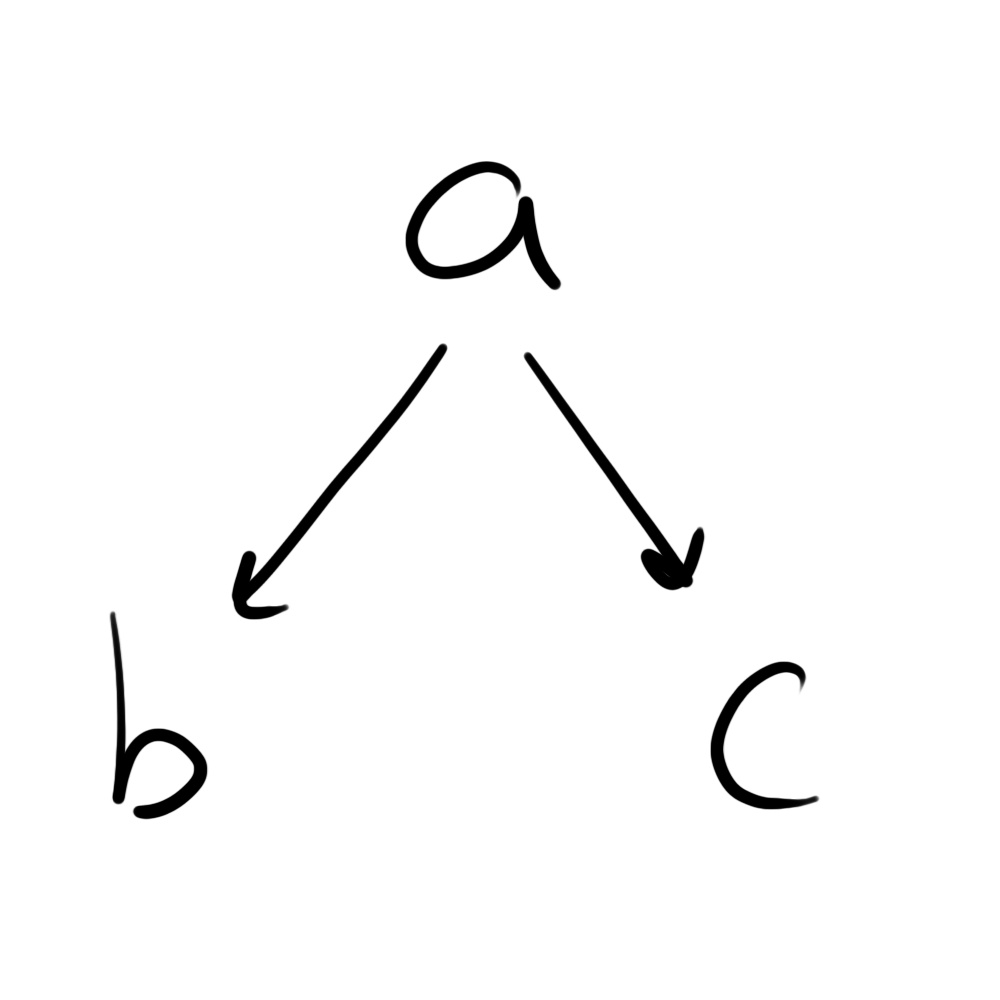
\includegraphics[scale=0.06]{gen1}
  \caption[] {
    \tabular[t]{@{}l@{}}
    $ARS = (A, R)$
    \\ $A = \{a, b, c\}$
    \\ $R = \{(a, b), (a, c)\}$
    \endtabular}
\end{figure}

\medskip\noindent
In figure 1, we obtain that our set of objects (A) consists of $a$, $b$, and $c$. We also see that our rules are that $a$ $\rightarrow$ $b$ and $a$ $\rightarrow$ $c$. These rules define the binary relationship between $a$, $b$, and $c$. Here is another example of a simple ARS:

\begin{figure}[h!]
  \centering
  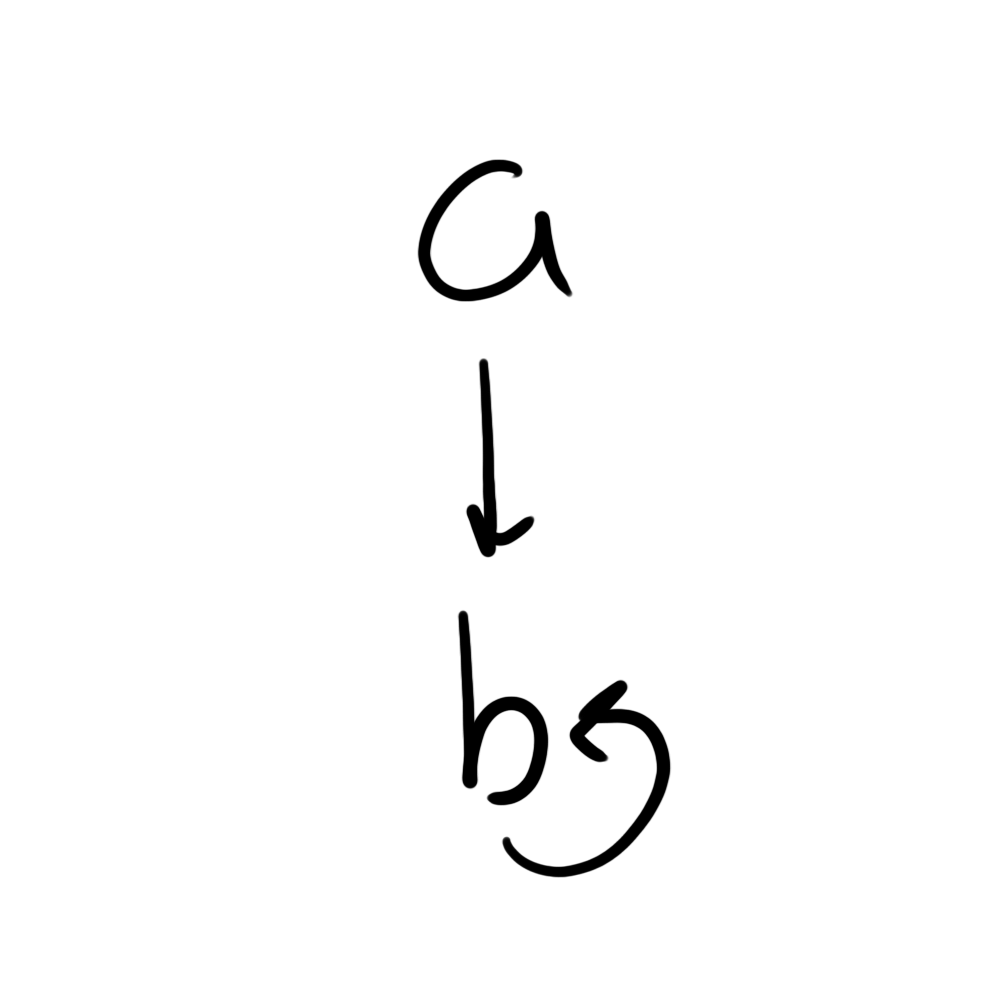
\includegraphics[scale=0.06]{gen2}
  \caption[] {
    \tabular[t]{@{}l@{}}
    $ARS = (A, R)$
    \\ $A=\{a,b\}$
    \\ $R=\{(a,b),(b,b)\}$
    \endtabular}
\end{figure}

\medskip\noindent
Figure 2's ARS is simple like the previous example, but now there is no $c$ object and $b$ loops back to itself. It is important to keep in mind that ARS's can loop. This topic will be explored later. There are an infinite amount of ARS examples that can be viewed for further exploration. For the purpose of keeping this overview brief, we will move on continue this exploration below.

\subsection{Significant Properties of Abstract Reduction Systems}

\subsubsection{Termination}

\medskip\noindent
One of the key properties of abstract reductions systems is termination. From basic intuition you may have guessed that if an ARS is terminating, then it will always stop at some point when executed. You would be correct to assume this. When there are no loops in an ARS, it will eventually terminate. It is rather simple to determine if the ARS will terminate since it is as simple as finding loops. Figures 3-8 visualize terminating and non-terminating ARS’s.

\begin{figure}[H]
  \centering
  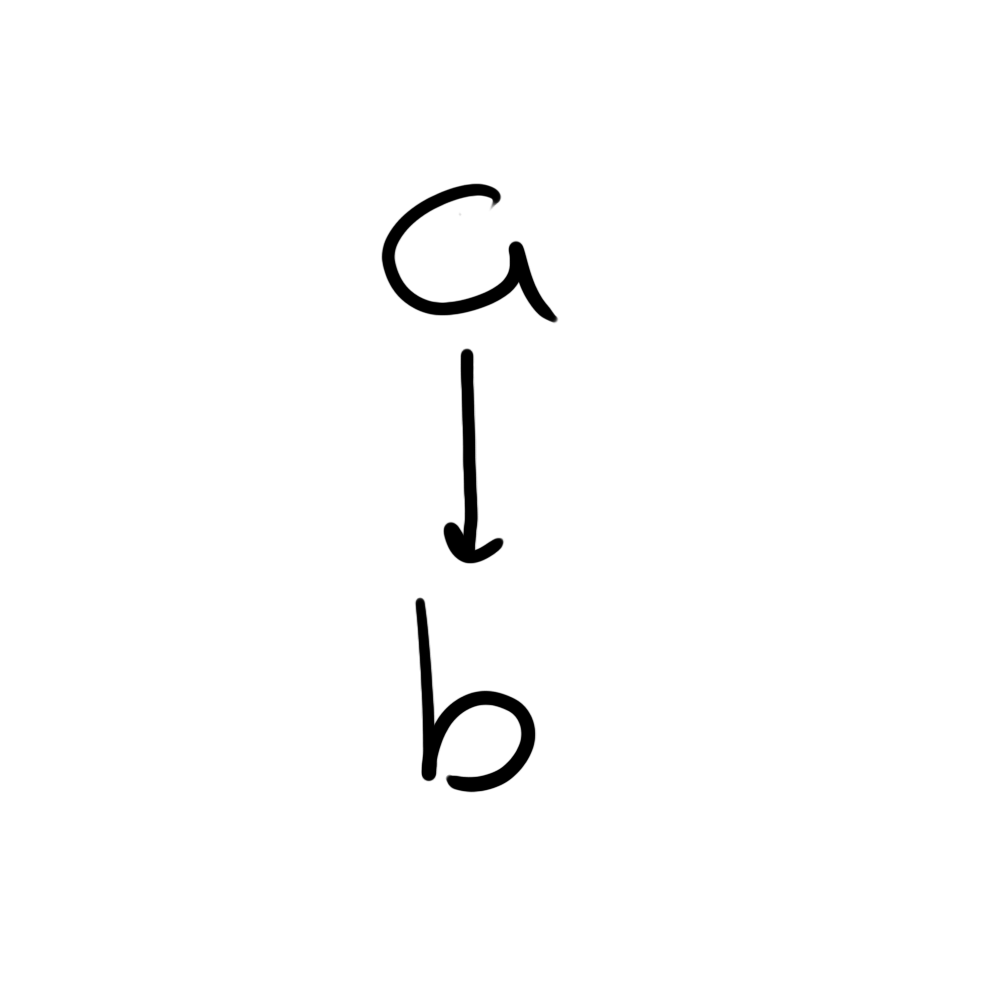
\includegraphics[scale=0.06]{gen3}
  \caption[] {
    \tabular[t]{@{}l@{}}
    $ARS = (A, R)$
    \\ $A=\{a,b\}$
    \\ $R=\{(a,b)\}$
    \endtabular}
\end{figure}

\begin{figure}[H]
  \centering
  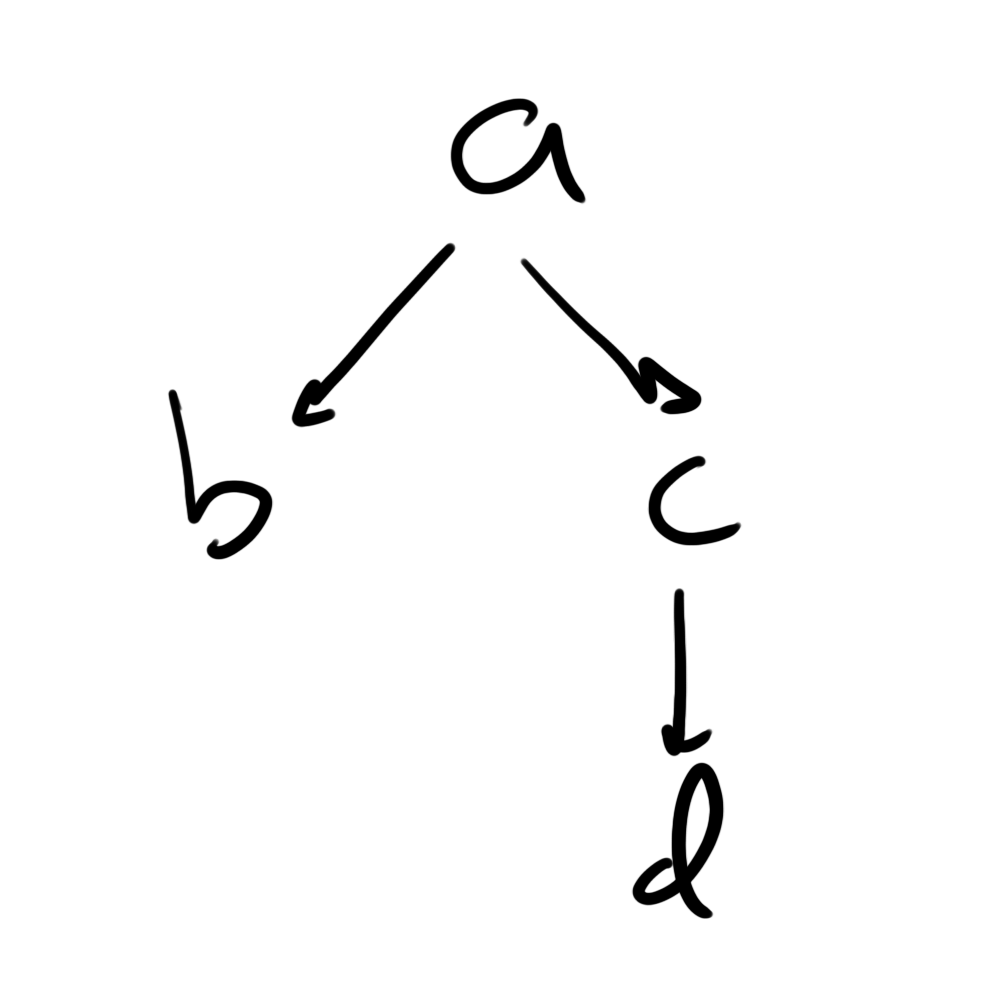
\includegraphics[scale=0.06]{gen4}
  \caption[] {
    \tabular[t]{@{}l@{}}
    $ARS = (A, R)$
    \\ $A=\{a, b, c, d\}$
    \\ $R=\{(a, b), (a, c), (c,d)\}$
    \endtabular}
\end{figure}

\begin{figure}[H]
  \centering
  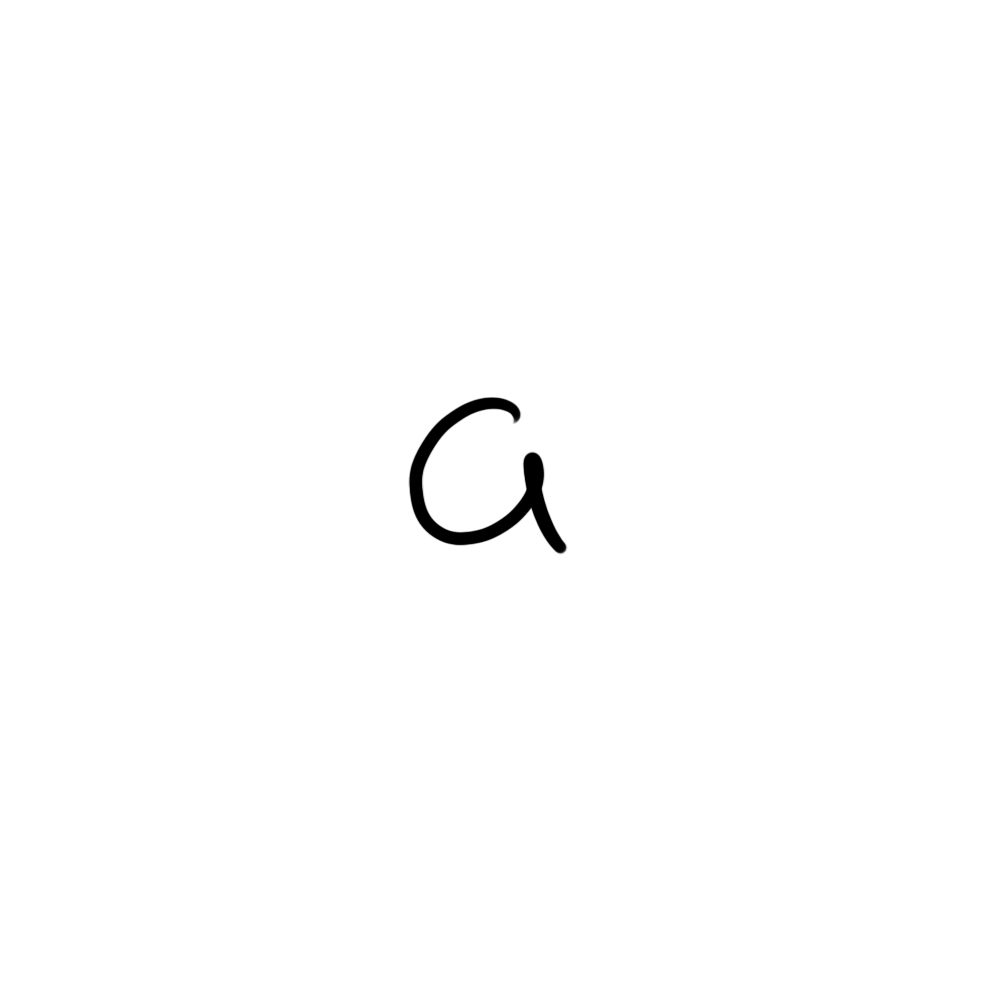
\includegraphics[scale=0.06]{gen5}
  \caption[] {
    \tabular[t]{@{}l@{}}
    $ARS = (A, R)$
    \\ $A=\{a\}$
    \\ $R=\{\}$
    \endtabular}
\end{figure}

\medskip\noindent
Note how in all of these examples above, the ARS reaches a definite end at some point. In figure 3, the ARS simply terminates at $b$. In figure 4, the ARS either terminates at $b$ or $d$. Lastly, figure 5, as simple as it is terminates at $a$. Therefore, all of these three ARS's terminating. Now we can explore what a non-terminating ARS looks like. Figures 6-8 below exemplify non-terminating ARS's.

\begin{figure}[H]
  \centering
  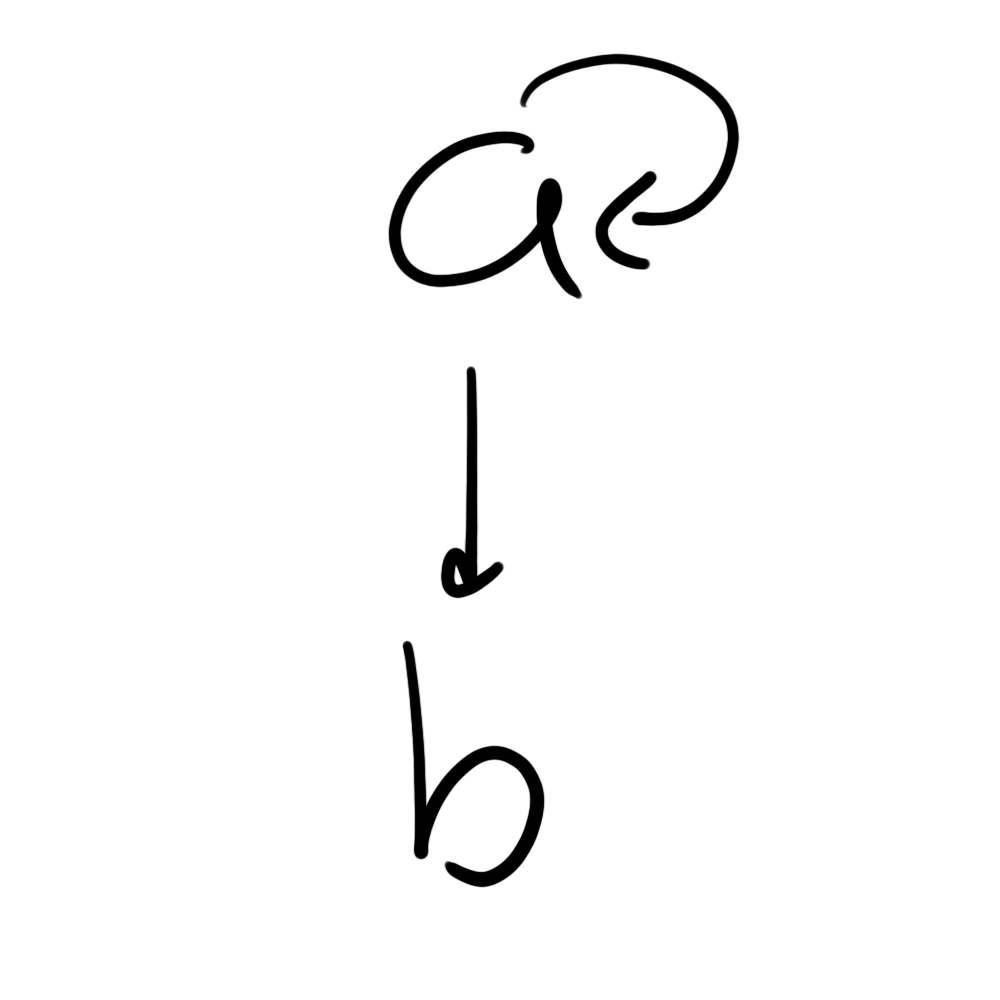
\includegraphics[scale=0.06]{gen6}
  \caption[] {
    \tabular[t]{@{}l@{}}
    $ARS = (A, R)$
    \\ $A=\{a, b\}$
    \\ $R=\{(a, a), (a, b)\}$
    \endtabular}
\end{figure}

\begin{figure}[H]
  \centering
  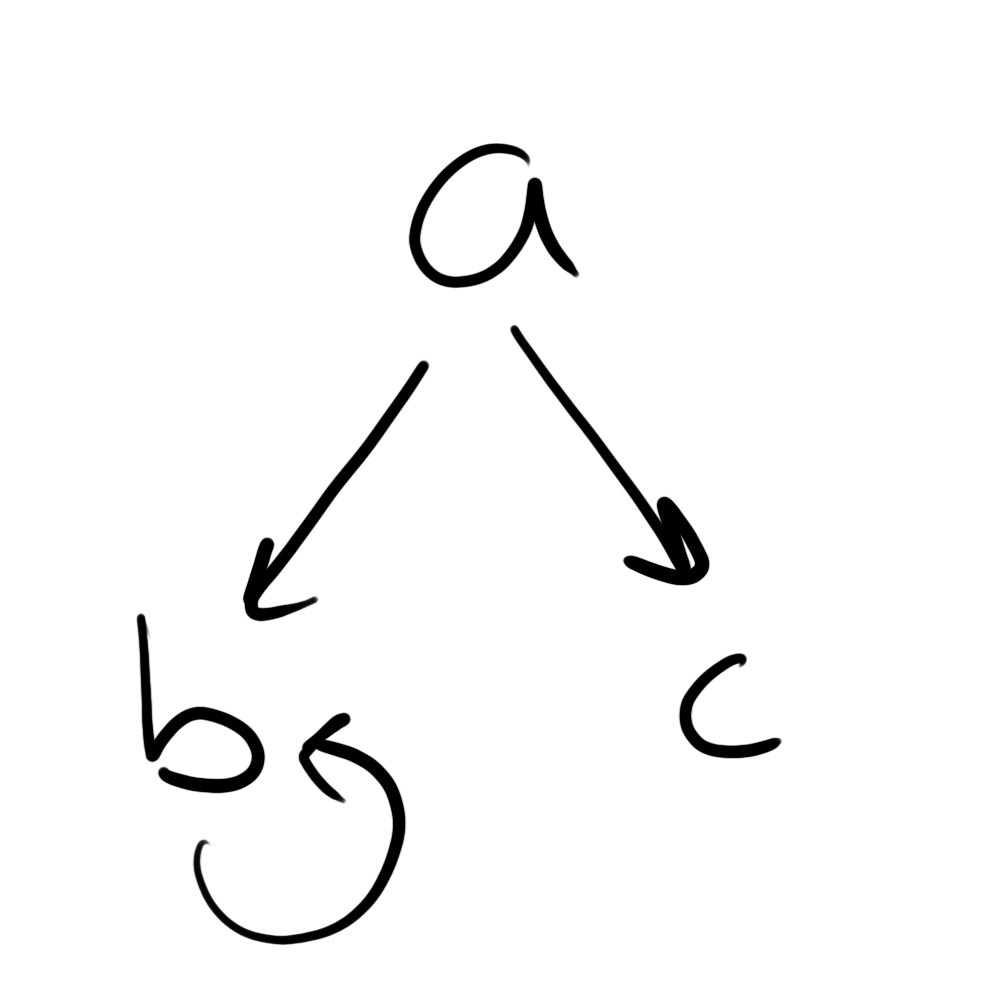
\includegraphics[scale=0.06]{gen7}
  \caption[] {
    \tabular[t]{@{}l@{}}
    $ARS = (A, R)$
    \\ $A=\{a, b, c\}$
    \\ $R=\{(a, b), (b, b), (a, c)\}$
    \endtabular}
\end{figure}

\begin{figure}[H]
  \centering
  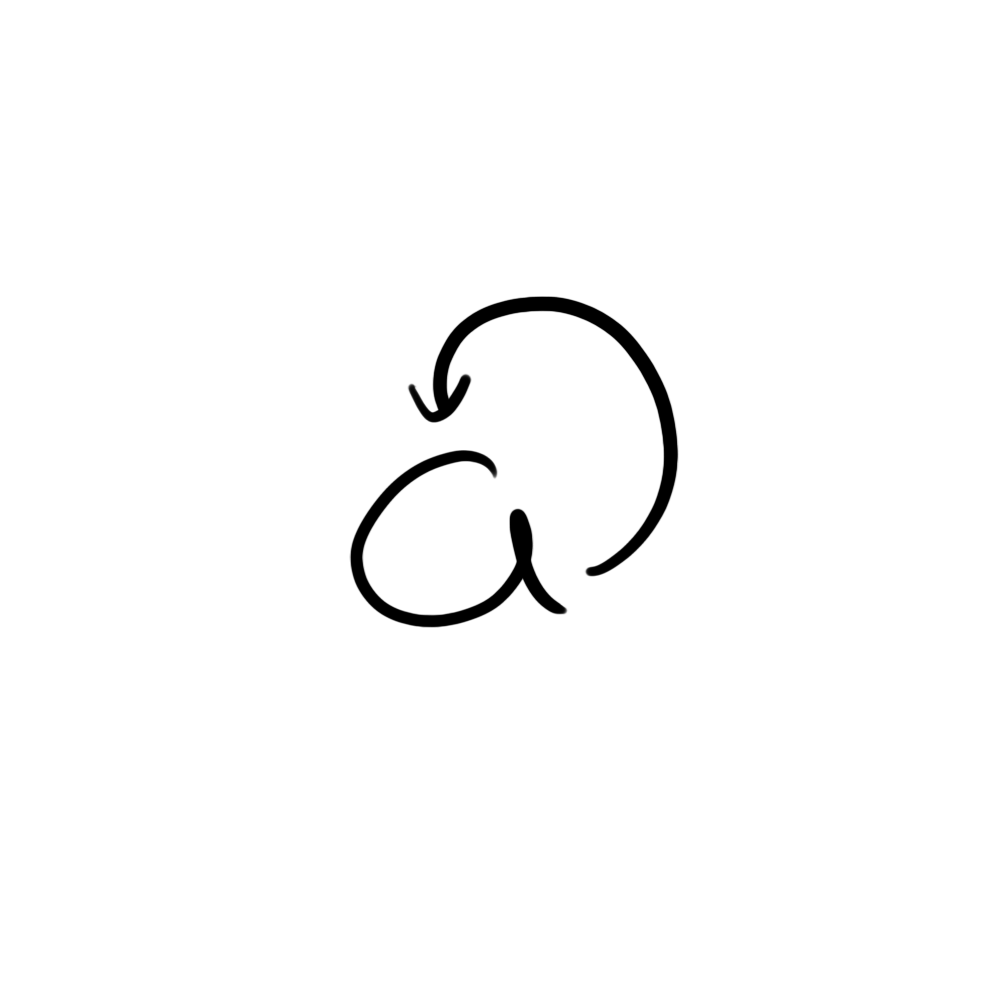
\includegraphics[scale=0.06]{gen8}
  \caption[] {
    \tabular[t]{@{}l@{}}
    $ARS = (A, R)$
    \\ $A=\{a\}$
    \\ $R=\{a, a\}$
    \endtabular}
\end{figure}

\medskip\noindent
Notice how in all of these examples there is a loop that prevents the ARS from completely terminating. In figure 6 and 8 the, $a$ loops to itself. In figure 7, $b$ does. Even if one path allows for termination, such as $b$ in figure 6 or $c$ in figure 7, the entire ARS would be considered non-terminating since there are portions where it could loop. When an ARS has a loop, it is non-deterministic, also meaning that it will not have the same result every time. In figure 6 for example, there is a possibility the ARS will simply terminate after reaching $b$. However, since there is also the possibility that the ARS would loop to object $a$, it is not deterministic, meaning that the possibility of looping forever nullifies the classification of terminating. Keep in mind that it is not only single-object loops that will do this. As long as there is some form of looping in the ARS, there will be non-termination. For example, in figure 6, if $a$ did not point to itself, but $b$ $\rightarrow$ $a$, the ARS would still be looping since $b$ loops back to $a$ which is the beginning of the ARS.


\subsubsection{Unique Normal Form (UNF)}

\medskip\noindent
To define a unique normal form, we must first define a normal form. A normal form is an object that no rules can apply to. This also implies that it is the end of the computation and can be recognized when there are no arrows stemming from the object. Figure 9 and 10 contain examples of normal forms:

\begin{figure}[H]
  \centering
  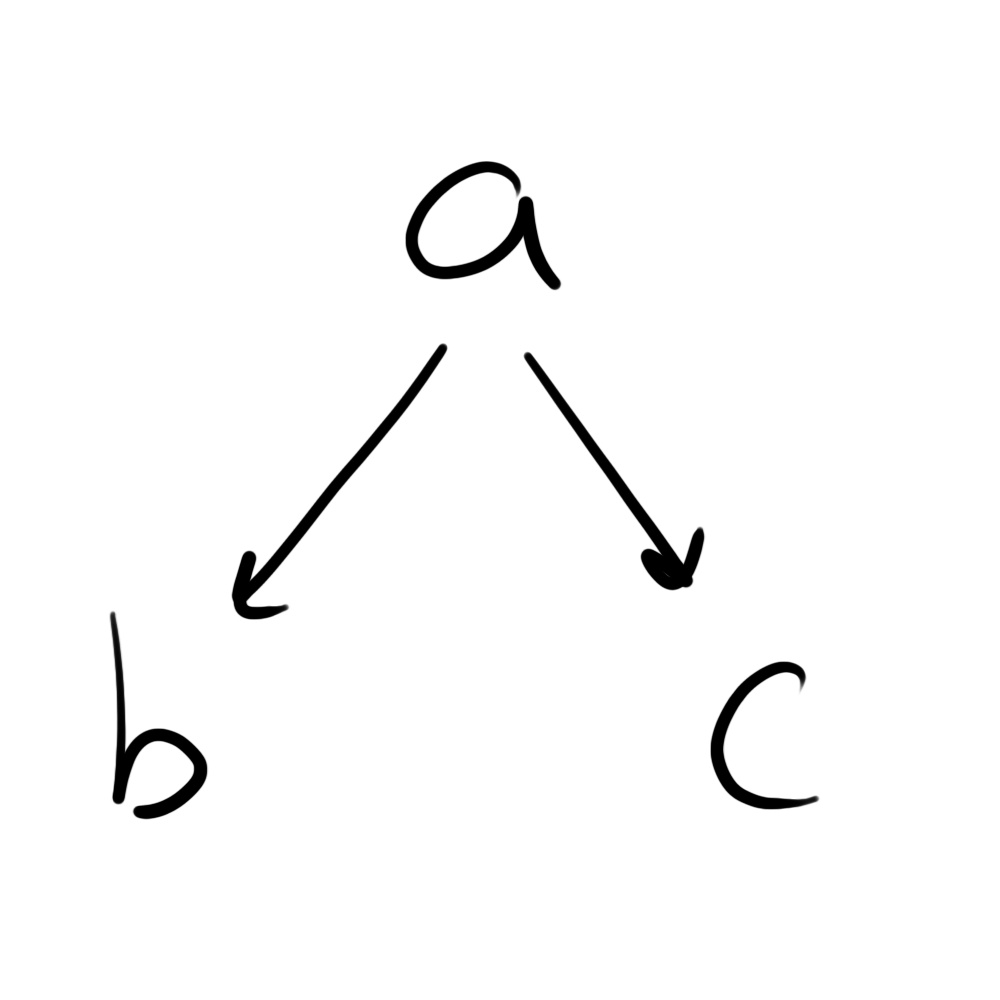
\includegraphics[scale=0.06]{gen9}
  \caption[] {
    \tabular[t]{@{}l@{}}
    $ARS = (A, R)$
    \\ $A=\{a, b, c\}$
    \\ $R=\{(a, b), (a, c)\}$
    \endtabular}
\end{figure}

\begin{figure}[H]
  \centering
  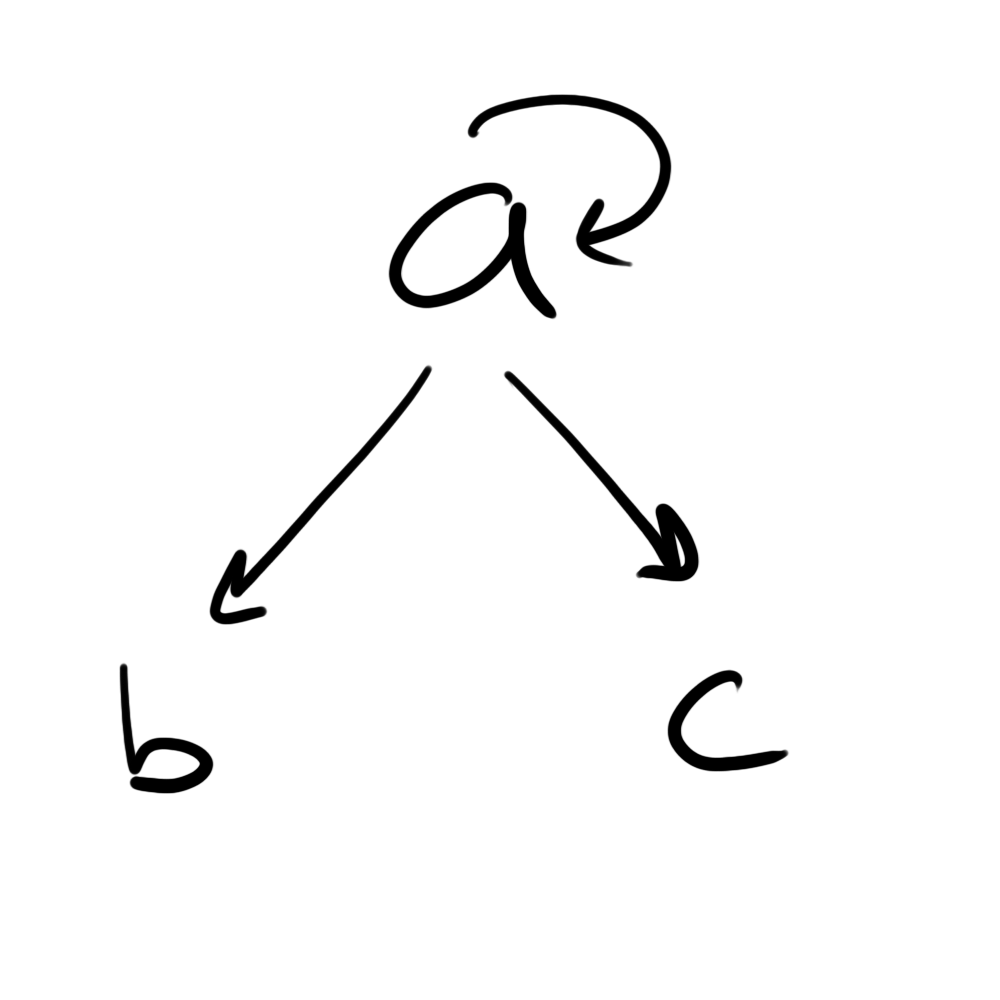
\includegraphics[scale=0.06]{gen10}
  \caption[] {
    \tabular[t]{@{}l@{}}
    $ARS = (A, R)$
    \\ $A=\{a, b, c\}$
    \\ $R=\{(a, a), (a, b), (a, c)\}$
    \endtabular}
\end{figure}

\medskip\noindent
As you may have guessed, the normal forms of figure 9 are both $b$ and $c$ because no rules can be applied to them. They are where the ARS terminates. In, figure 10, it is the same, despite having $a$ looping. An ARS does not need to be terminating in order to contain a normal form. The relationships of all of these significant properties will be covered later. For now we will move onto unique normal forms.

\medskip\noindent
A unique normal form (UNF) is the same thing as a normal form, except it must be the one and only occuring normal form of the ARS. It is called the “unique” normal form because the ARS will only have one. Figure 11-13 contain examples of unique normal forms:

\begin{figure}[H]
  \centering
  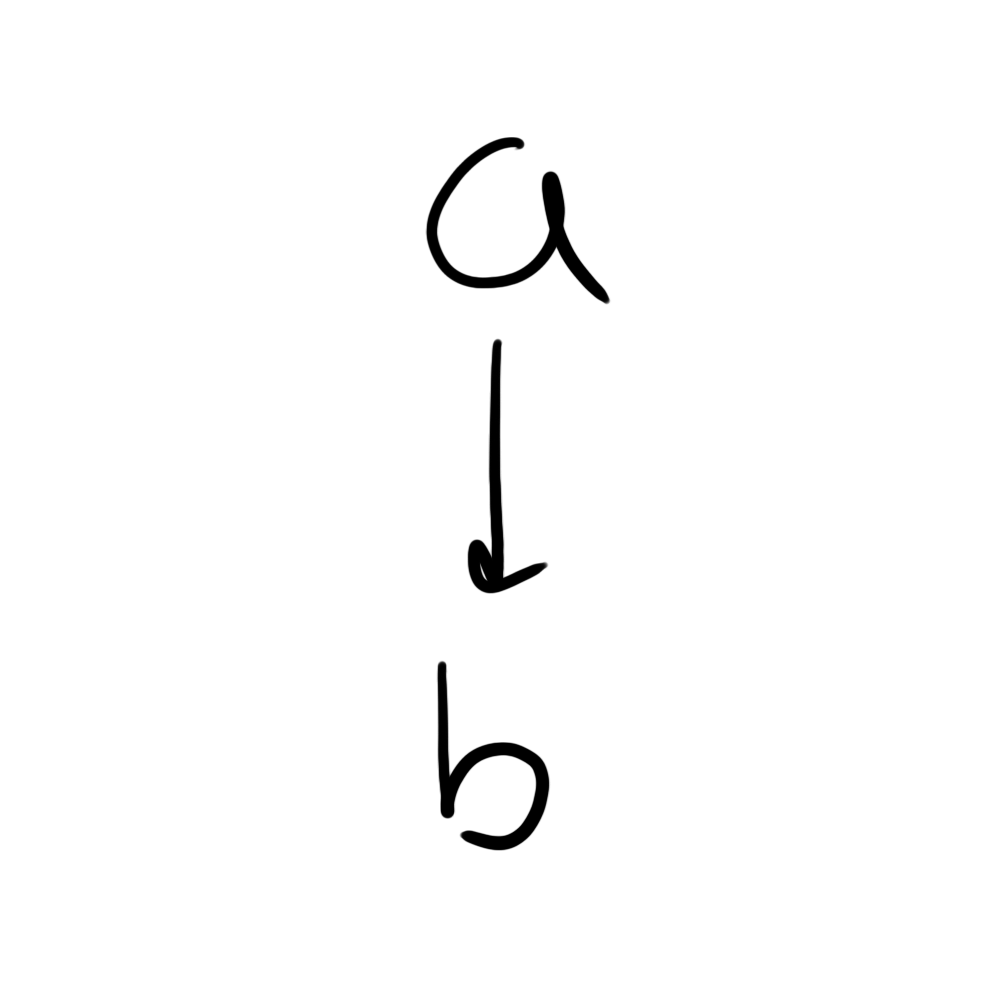
\includegraphics[scale=0.06]{gen11}
  \caption[] {
    \tabular[t]{@{}l@{}}
    $ARS = (A, R)$
    \\ $A=\{a, b\}$
    \\ $R=\{(a, b)\}$
    \endtabular}
\end{figure}

\begin{figure}[H]
  \centering
  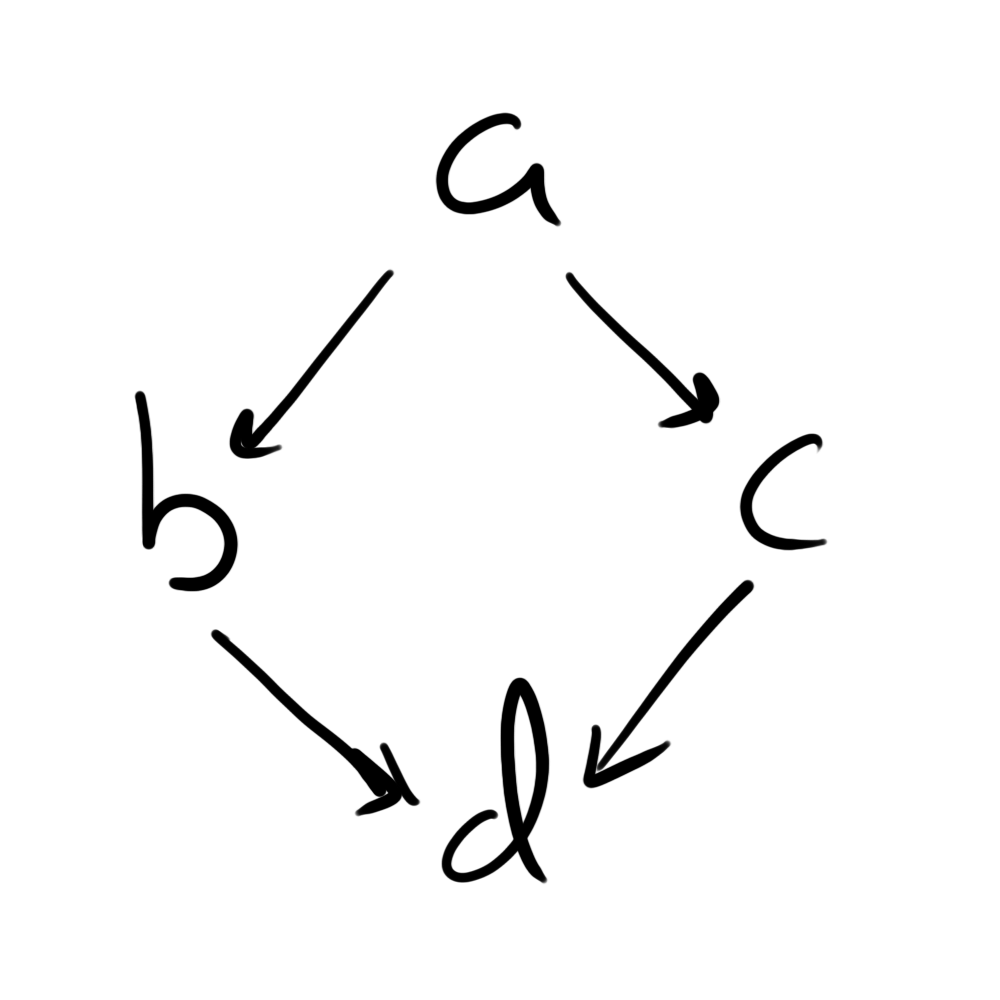
\includegraphics[scale=0.06]{gen12}
  \caption[] {
    \tabular[t]{@{}l@{}}
    $ARS = (A, R)$
    \\ $A=\{a, b, c, d\}$
    \\ $R=\{(a, b), (a, c), (b, d), (c, d)\}$
    \endtabular}
\end{figure}

\begin{figure}[H]
  \centering
  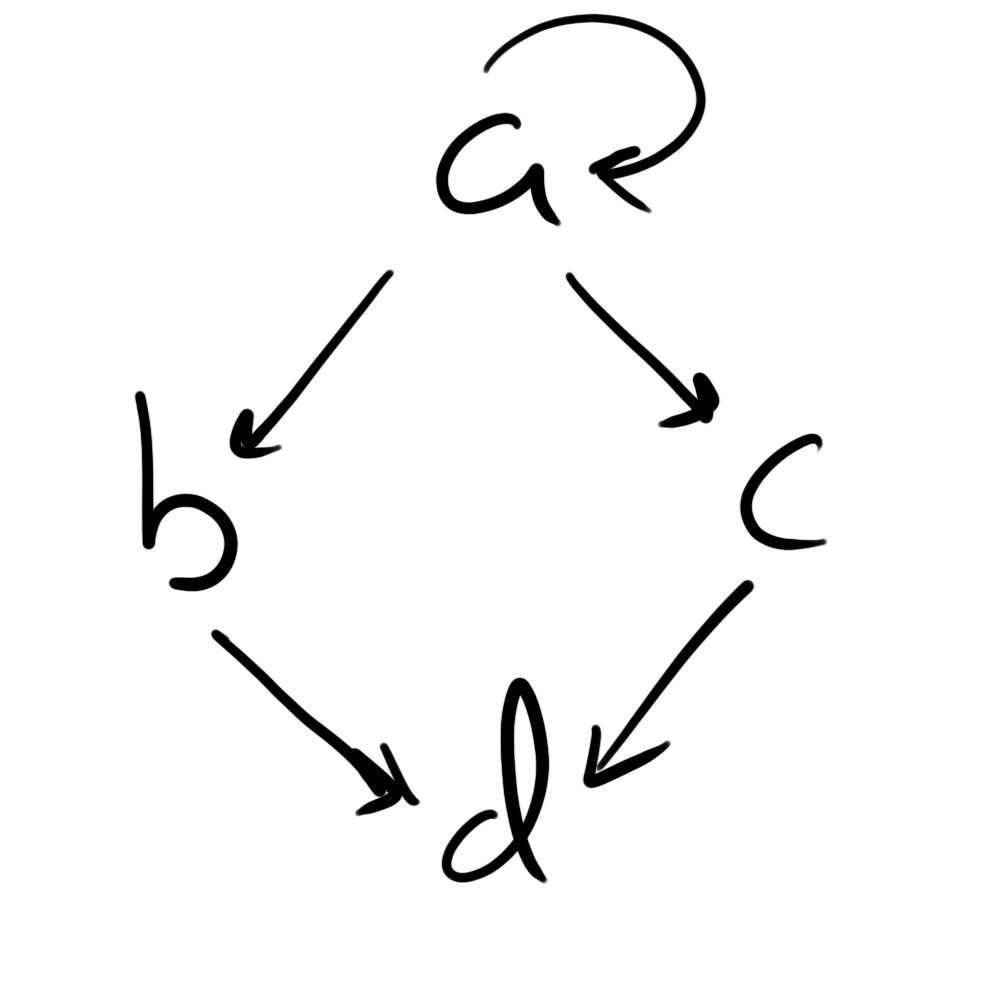
\includegraphics[scale=0.06]{gen13}
  \caption[] {
    \tabular[t]{@{}l@{}}
    $ARS = (A, R)$
    \\ $A=\{a, b, c, d\}$
    \\ $R=\{(a, a), (a, b), (a, c), (b, d), (c, d)\}$
    \endtabular}
\end{figure}

\medskip\noindent
As you can see, both of these examples reveal that each ARS leads a UNF. In figure 11 it is $b$. In figure 12 and 13 it is $d$. Keep in mind that having a UNF does not imply that the ARS will be deterministic, since there can be a UNF in an ARS with loops. Figure 13 is an example of this.


\subsubsection{Confluence}

\medskip\noindent
An ARS is confluent if for every peak, there is a valley. In the familiar ARS represented in figure 14, $(a, b)$ and $(a, c)$ represent the peak and $(b, d)$ and $(c, d)$ represent the valley.

\begin{figure}[H]
  \centering
  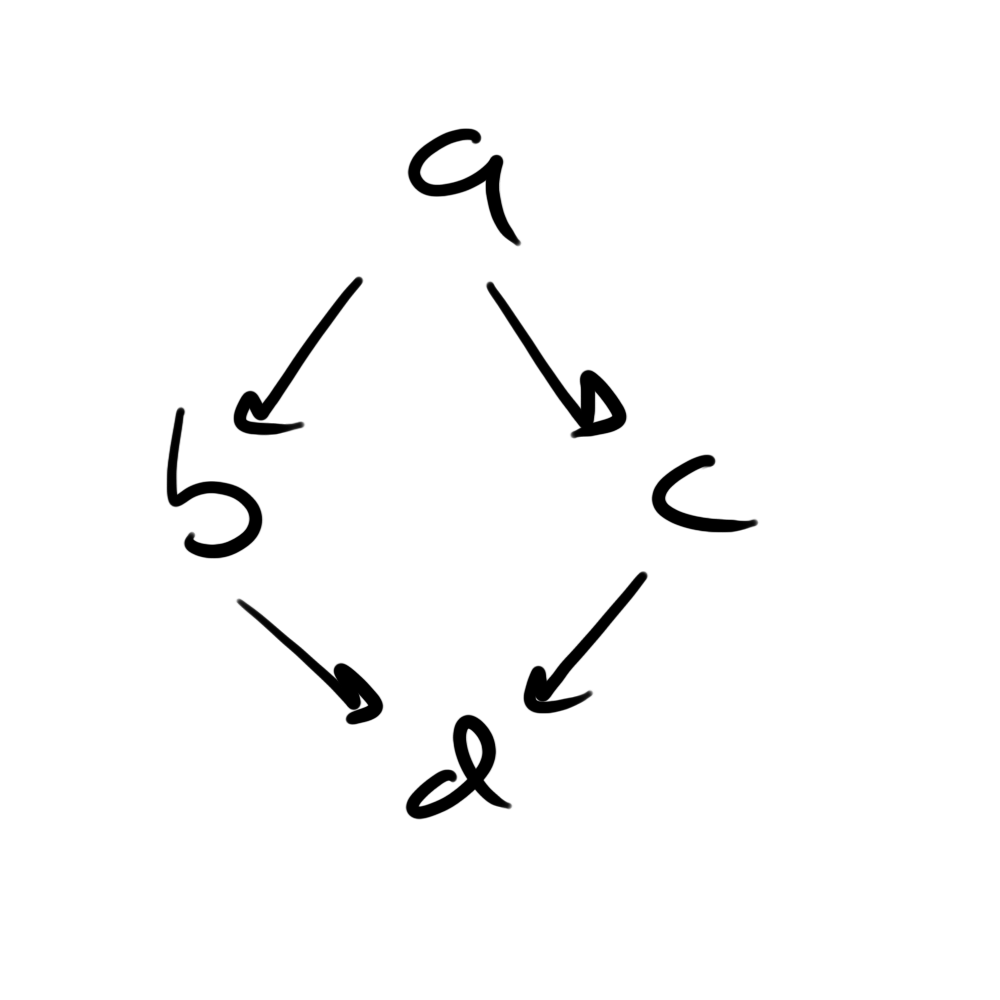
\includegraphics[scale=0.06]{gen14}
  \caption[] {
    \tabular[t]{@{}l@{}}
    $ARS = (A, R)$
    \\ $A=\{a, b, c, d\}$
    \\ $R=\{(a, b), (a, c), (b, d), (c, d)\}$
    \endtabular}
\end{figure}

\medskip\noindent
If the ARS can take multiple routes to achieve the same result, then it is confluent. Confluence can be seen in figure 14 since both routes $(a \rightarrow b \rightarrow d)$ and $(a \rightarrow c \rightarrow d)$ lead to the same result. Here are more examples of confluent ARS's.

\begin{figure}[H]
  \centering
  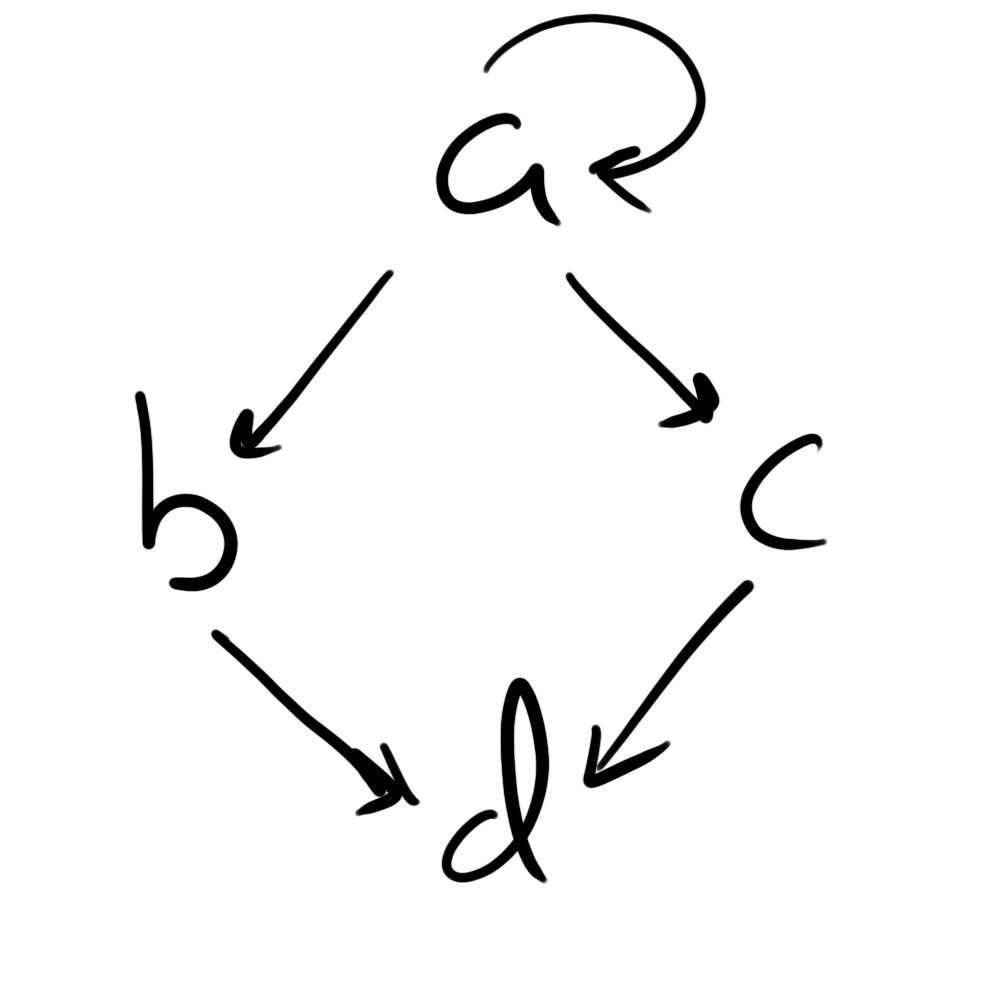
\includegraphics[scale=0.06]{gen15}
  \caption[] {
    \tabular[t]{@{}l@{}}
    $ARS = (A, R)$
    \\ $A=\{a, b, c, d\}$
    \\ $R=\{(a, a), (a, b), (a, c), (b, d), (c, d)\}$
    \endtabular}
\end{figure}

\begin{figure}[H]
  \centering
  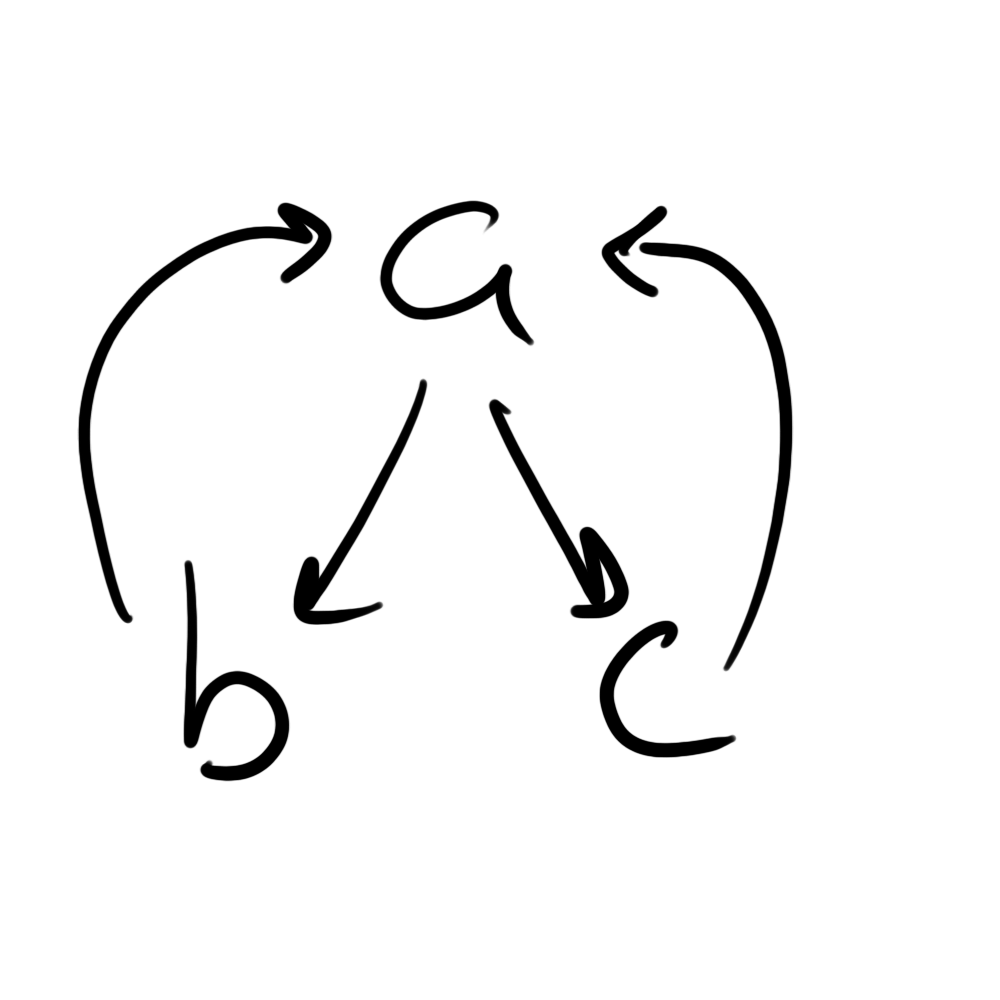
\includegraphics[scale=0.06]{gen16}
  \caption[] {
    \tabular[t]{@{}l@{}}
    $ARS = (A, R)$
    \\ $A=\{a, b, c\}$
    \\ $R=\{(a, b), (a, c), (b, a), (c, a)\}$
    \endtabular}
\end{figure}

\medskip\noindent
The ARS in figure 15 is almost identical to figure 14's. However, $a$ loops to itself, making the ARS non-terminating. This shows that confluent ARS's do not need to be terminating. As long as the ARS can take multiple routes to achieve the same result, it is confluent. Confluence  is not nullified if the ARS contains a loop, unlike termination. Moving on, the confluent ARS in figure 16 contains a more complex loop as $b$ and $c$ both loop back to $a$. The corresponding valley for the peak, $(a, b)$ and $(a, c)$, may not seem as obvious, the multiple routes of the ARS lead to the same object, which in this case is $a$, making it confluent.

\subsection{Relationships Between the Properties of Abstract Reduction Systems}

\medskip\noindent
Though we have covered some of the basic relationships between confluence, termination, and unique normal forms, there is still much to discover in terms of the combinations of the three. More specifically, you may have suspected that not all combinations of these three properties are possible in ARS’s.

\medskip\noindent
Here is a chart with corresponding ARS's to help visualize these relationships. Keep in mind that other ARS's can apply to some of relationship combinations. These are just some of the simple ARS's that we have already covered. Note that the ARS's are color coded with the chart. The rows in the chart without color are the combinations that require some further debate and theory to prove whether or not they can exist as abstract reduction systems.

\begin{figure}[h!]
  \centering
  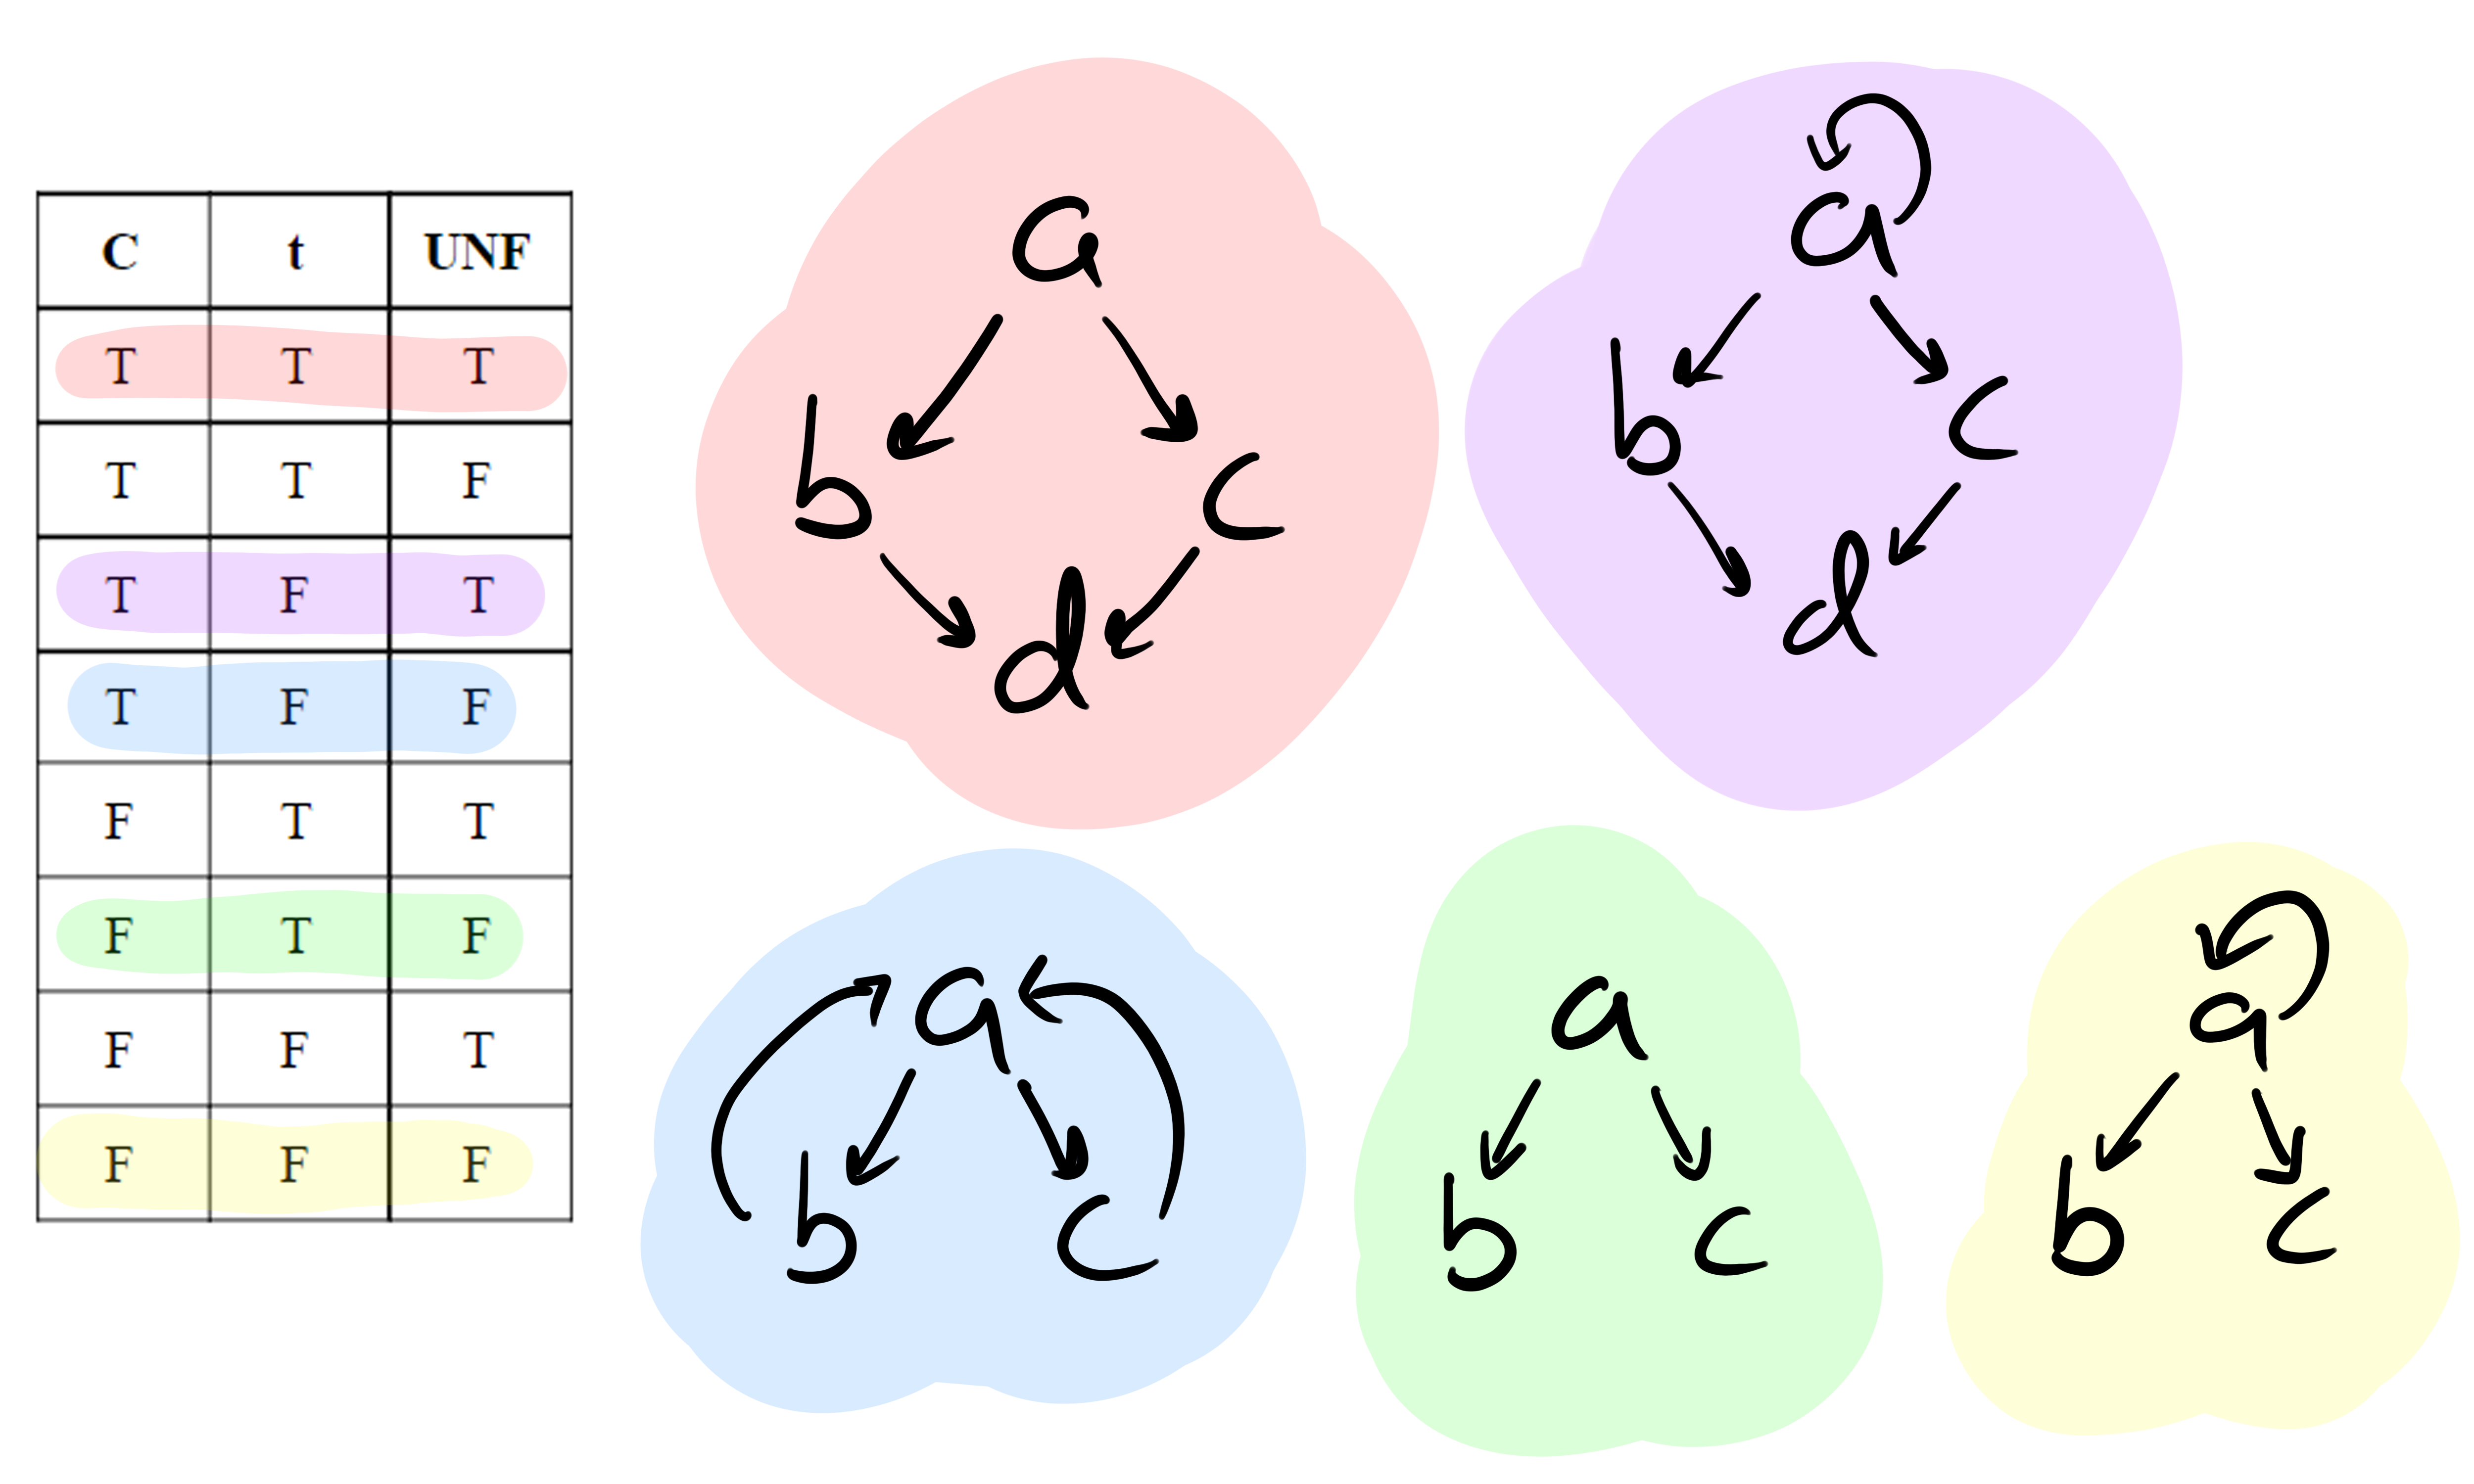
\includegraphics[scale=0.06]{arsComparisonGen}
\end{figure}

\medskip\noindent
Some of the cases that you may have encountered are that if an ARS is confluent and terminating, then it must have a UNF. Similarly, if an ARS is not confluent and then it cannot have a UNF. These relationships can be expressed in mathematical boolean notation:

\medskip
  $\neg$ (C $\land$ T $\land$ $\neg$ UNF)

\medskip
  $\neg$ ($\neg$ C $\land$ T $\land$ UNF)

\medskip
  $\neg$ ($\neg$ C $\land$ $\neg$ T $\land$ UNF)

\medskip\noindent
With boolean algebra, this can eventually be simplified to:

\medskip
  C $\lor$ $\neg$ UNF

\medskip\noindent
Which implies:

\medskip
  UNF $\Rightarrow$ C

\medskip\noindent
For reference, here is what the boolean notation would look like in C code:

\begin{lstlisting}[style=CStyle]
  !(C && T && !UNF)
  !(!C && T && UNF)
  !(!C && !T && UNF)
\end{lstlisting}

\medskip\noindent
Again, this can be simplified to:

\begin{lstlisting}[style=CStyle]
  C || !UNF
\end{lstlisting}

\medskip\noindent
Which again reveals that UNF implies confluence.


\subsection{Visualizing Reflexive, Symmetric, and Transitive Traits}

\medskip\noindent
For this tutorial we will be pairing two methods of visualizing abstract reduction systems. For each example, the first visualization will be a new way of representing the ARS's. The ARS's objects will be listed in alphabetic order in two identical columns \cite{RST}. Keep in mind that these columns are duplicates. They are the same exact objects, just mirrored. The relations between the objects will be represented by arrows going from the left column to the right. Furthermore, the second form of visualization for eachg example will simply be the same types of drawings that have been used for the prior theory portion this report.

\medskip\noindent
The purpose of this is to help understand reflexivity, symmetry, and transitivity by providing an additional form of visualization. Comparing these two forms of visualization should make it easier to grasps these concepts. Keep in mind that the color blue will be used to express changes to the visualzations.

\subsubsection{Visualizing Reflexivity}

\medskip\noindent
Consider this ARS as both a two-column and traditional visualization in figures 17 and 18:

\medskip\noindent
First, it may be helpful to compare the two kinds of visualizations. Pay close attention to how in both figures the relations between the objects are the same. For example consider $a$. In figure 17 it points to $a$ and $c$, but to its mirrored right hand column. In the traditional example, it is exactly the same, however, there is no mirror. $a$ simply points to its non-mirrored self as a loop and also points to the non-mirrored version of $c$. Also, the location of the objects is more 2-dimensional compared to the columns.

\begin{figure}[H]\
  \centering
  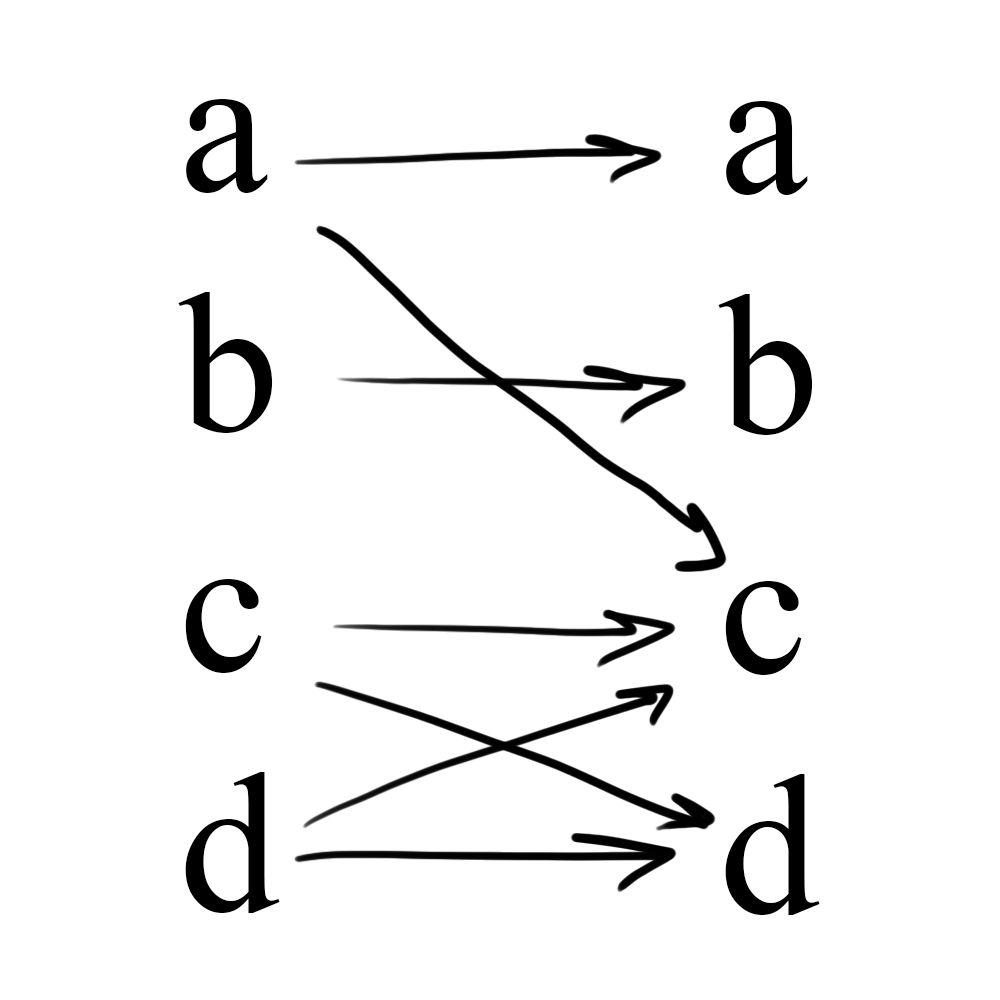
\includegraphics[scale=0.06]{s1}
  \caption[] {
    \tabular[t]{@{}l@{}}
    Two-column visualization of (A, R)
    \\ $A = \{a, b, c ,d\}$
    \\ $R = \{(a, a), (a, c), (b, b), (c, c) (c, d), (d, d), (d, c)\}$
    \endtabular}
\end{figure}

\begin{figure}[H]
  \centering
  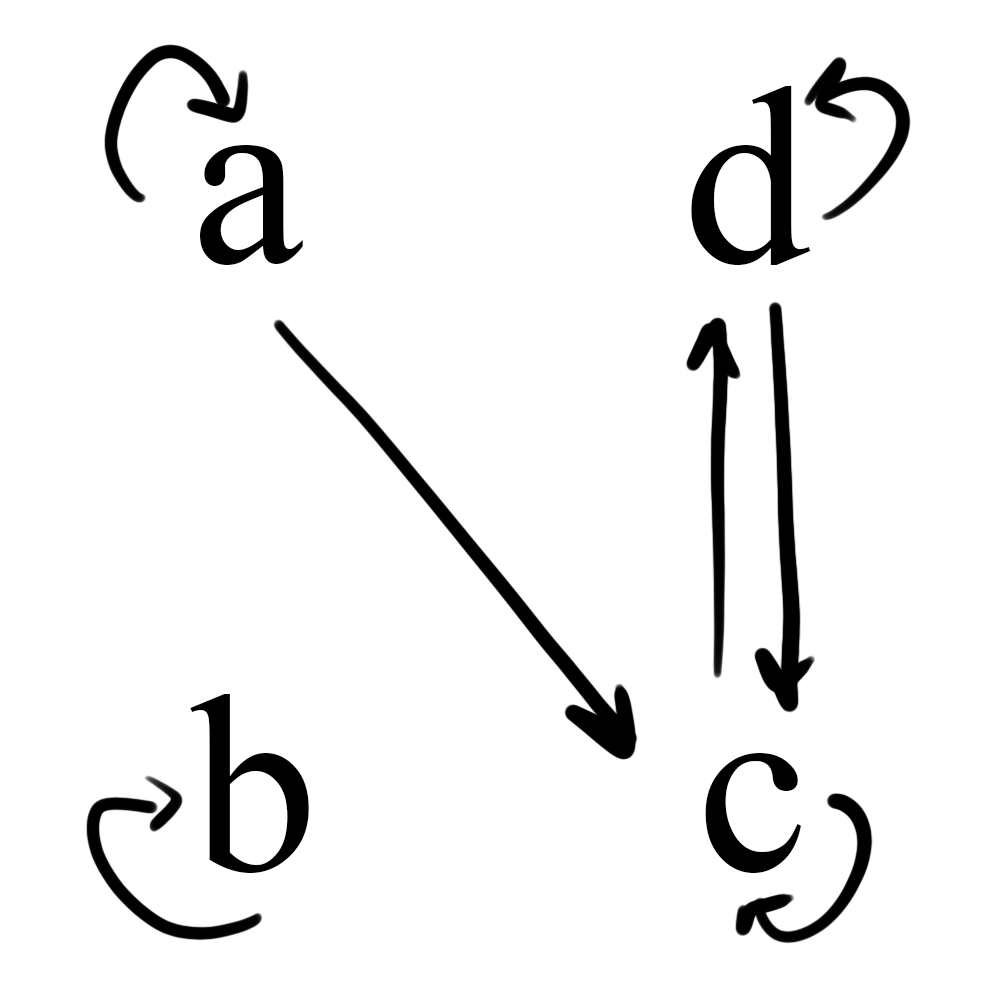
\includegraphics[scale=0.06]{v1}
  \caption[] {
    \tabular[t]{@{}l@{}}
    The same ARS shown in figure 17 but visualized traditionally.
    \endtabular}
\end{figure}

\medskip\noindent
Now that we fully understand these differences between the two visualization types, we can finally discuss reflexivity within abstract reduction systems. When an object points to itself, it is reflexive. In this example, every object is reflexive. This means that the entire set, $A$, is reflexive. However, if just one element did not point to itself, then the entire A could not be considered reflexive.

\subsubsection{Visualizing Symmetry}

\medskip\noindent
Taking a look at the prior ARS from Figure 17, notice how the lower portion of the set $A$ appears to be symmetric. This is because not only does $c \rightarrow d$, but $d \rightarrow c$ too. Therefore there is symmetry between these $c$ and $d$. However, since the entire set $A$ is not symmetric, the set is considered asymmetrical. Now we will change that prior example to make the set fully reflexive. To do this we would have to make $c \rightarrow a$. The modifications can be seen in figures 19 and 20 below:

\begin{figure}[H]
  \centering
  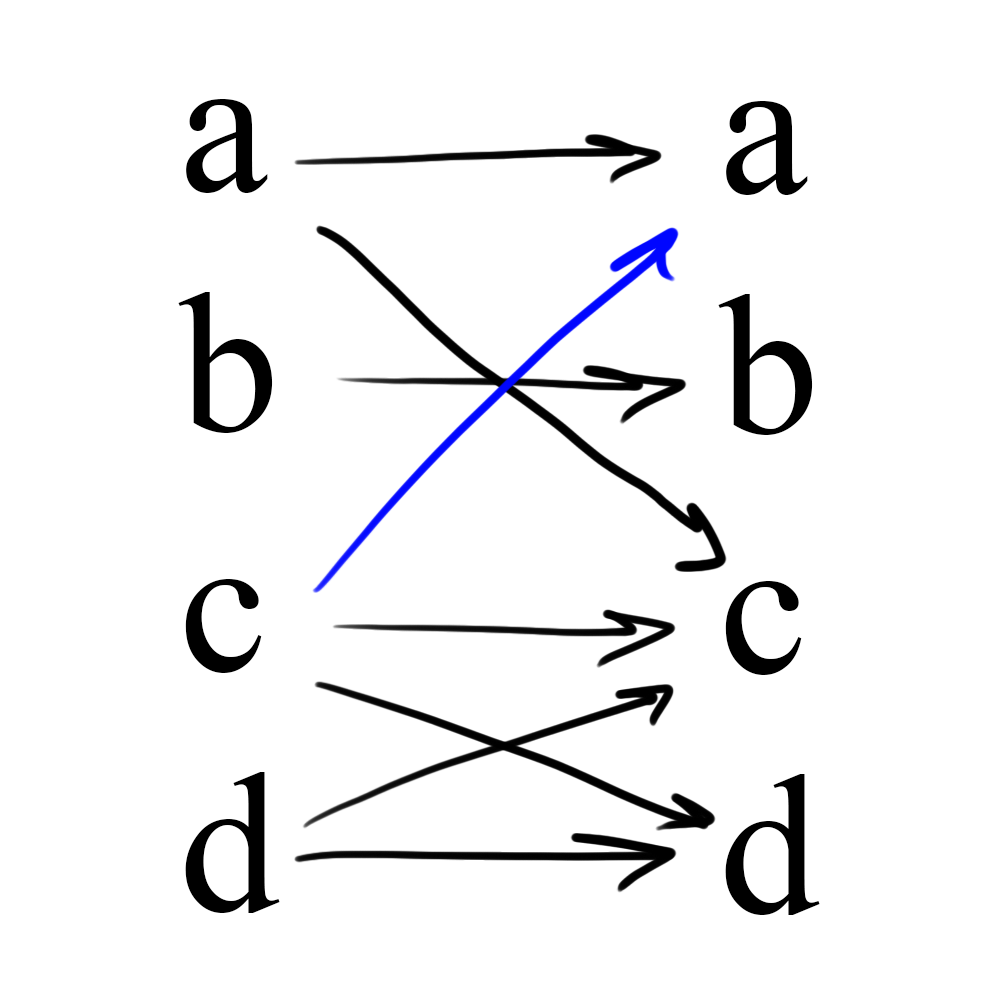
\includegraphics[scale=0.06]{s3}
  \caption[] {
    \tabular[t]{@{}l@{}}
    Symmetric two-column visualization of set A where,
    \\ $ARS = (A, R)$
    \\ $A = \{a, b, c ,d\}$
    \\ $R = \{(a, a), (a, c), (b, b), (c, c), (c, a), (c, d), (d, d), (d, c)\}$
    \endtabular}
\end{figure}

\begin{figure}[H]
  \centering
  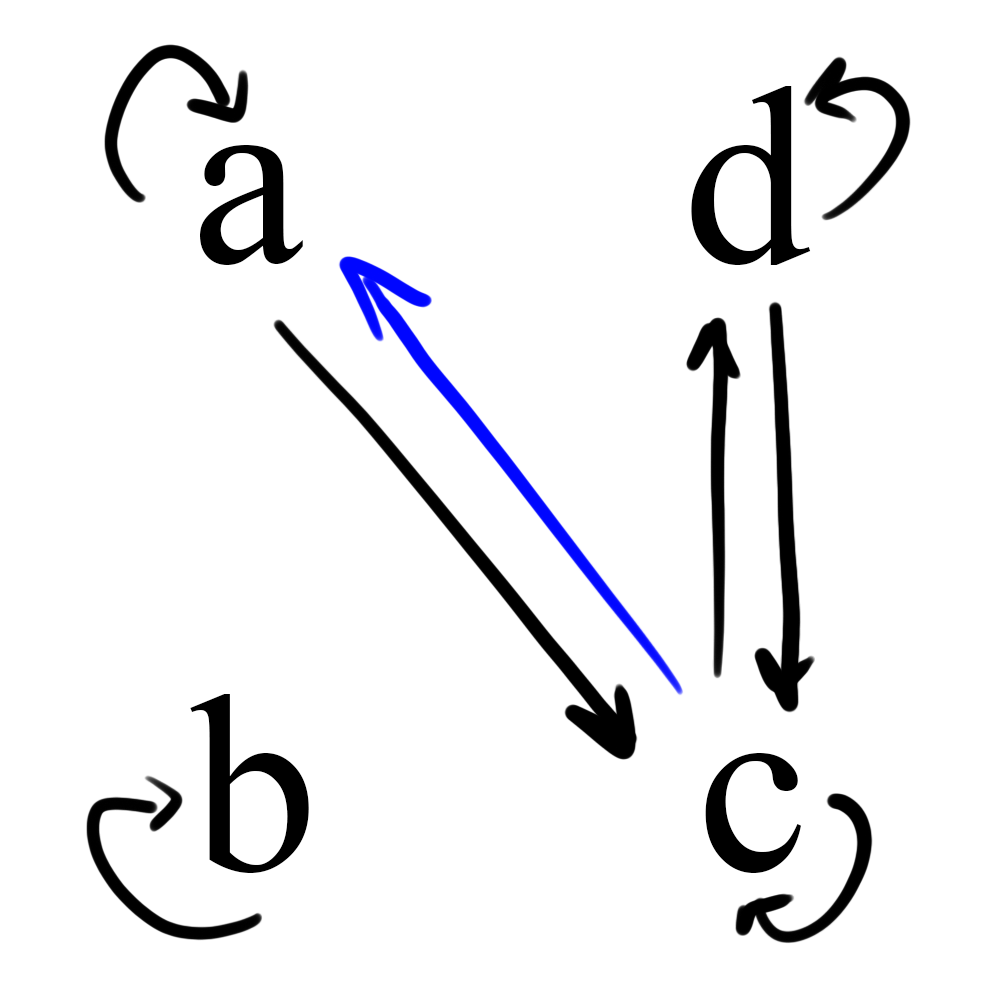
\includegraphics[scale=0.06]{v2}
  \caption[] {
    \tabular[t]{@{}l@{}}
    Traditional visualization of the modified ARS in figure 19.
    \endtabular}
\end{figure}
    
\medskip\noindent
With the 2 column visualization of the set in figure 19, it is easy to see if it is symmetric because the drawing itself will almost be completely symmetrical. The only aesethetically asymmetric aspect of the drawing is that when an object is reflexive and is pointing to itself, it does not appear to point back. Keep in mind that it is also symmetric because it is simply pointing to itself.

\medskip\noindent
Notice how in the traditional visualization in figure 20, there are arrows going both to and from $a$ and $b$, and also $c$ and $d$. This can be rewritten with the proper notation using $\longleftrightarrow$. The ARS with corrected symbolic notation would look like:

\begin{figure}[H]
  \centering
  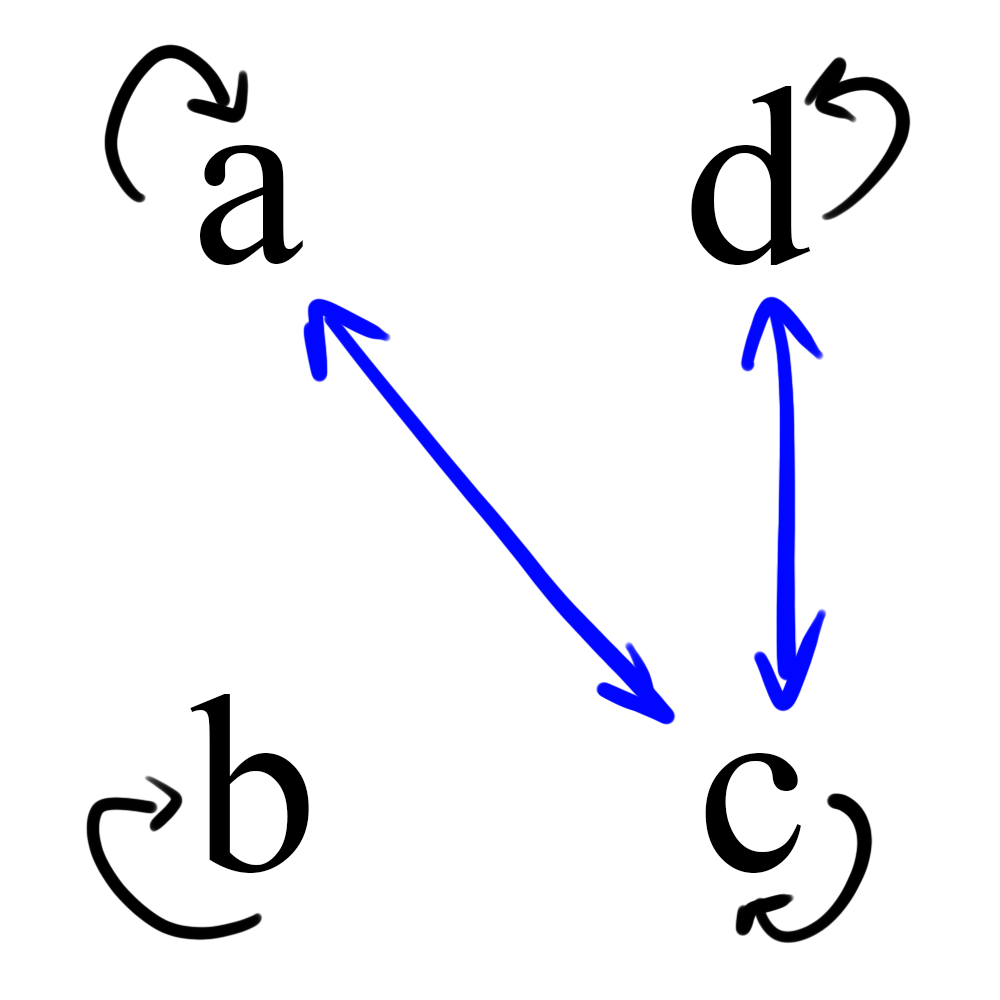
\includegraphics[scale=0.06]{v3}
  \caption[] {
    \tabular[t]{@{}l@{}}
    $(A, R)$ with proper notation
    \endtabular}
\end{figure}

\subsubsection{Visualizing Transitivity}

\medskip\noindent
Transitivity tends to feel more complicated compared to reflexivity and symmetry. To understand the general idea of transitivity, it is helpful to think of shortcuts. For example, lets just say you are in your room and are trying to reach the kitchen. In order to do so, you would have to walk down a hallway from your room to the living room. From the living room, you would walk down second hallway to finally reach the kitchen. This would be a two-step process. Now imagine there is a shortcut hallway that allows you to go directly from your room to the kitchen. This is a one-step process. Not only would the shortcut be transitive, but the entire system of your room, living room, and kitchen would be too (considering that you only have those three rooms). This is because of the aspect that allows you to reach the same position from either the original route, or the new shortcut.

\medskip\noindent
In figures 22-25 we will visualize this transitivity with our new and traditional ARS visualizations. Figure 22 and 23 will represent the opportunity of transivitiy before the modification has been made. Figures 24 and 25 will show the modifications that make the ARS transitive. If you wish to keep the bedroom/kitchen analogy in mind, think of $a$ as the bedroom, $c$ as the living room, and $d$ as the kitchen.

\begin{figure}[H]
  \centering
  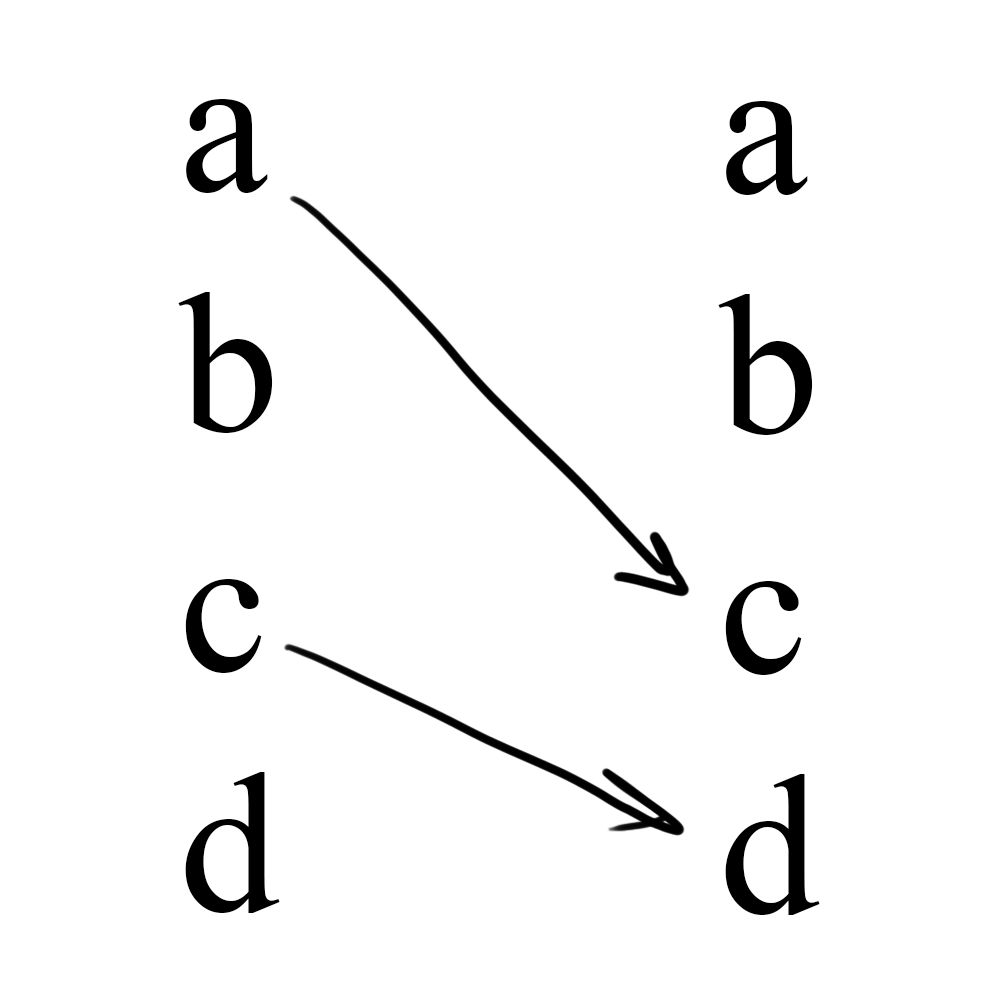
\includegraphics[scale=0.06]{s4}
  \caption[] {
    \tabular[t]{@{}l@{}}
    $ARS = (A, R)$
    \\ $A = \{a, b, c ,d\}$
    \\ $R = \{(a, c), (c, d)\}$
    \endtabular}
\end{figure}

\begin{figure}[H]
  \centering
  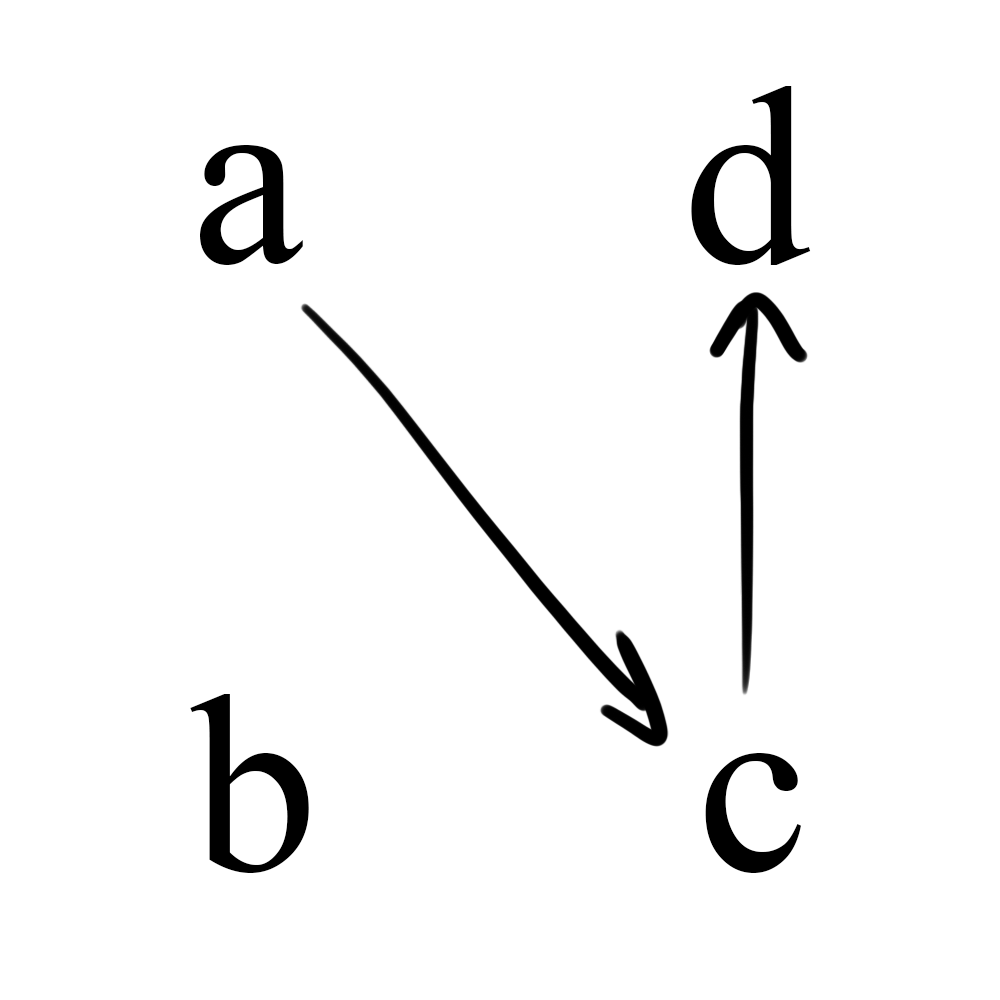
\includegraphics[scale=0.06]{v4}
  \caption[] {
    \tabular[t]{@{}l@{}}
    Traditional visualization of figure 22.
    \endtabular}
\end{figure}

\medskip\noindent
In figure 22, notice how $a \rightarrow c$ and $c \rightarrow d$. Shouldn’t that mean that there could be a shortcut from $a \rightarrow d$? If this shortcut was added, and the relations were updated to $R = \{(a, c), (a, d), (c, d)\}$ then the ARS would be transitive. The notation for this shortcut relation would be: $\xrightarrow{+}$. The modified versions with proper notation can be seen below in figures 24 and 25:

\begin{figure}[H]
  \centering
  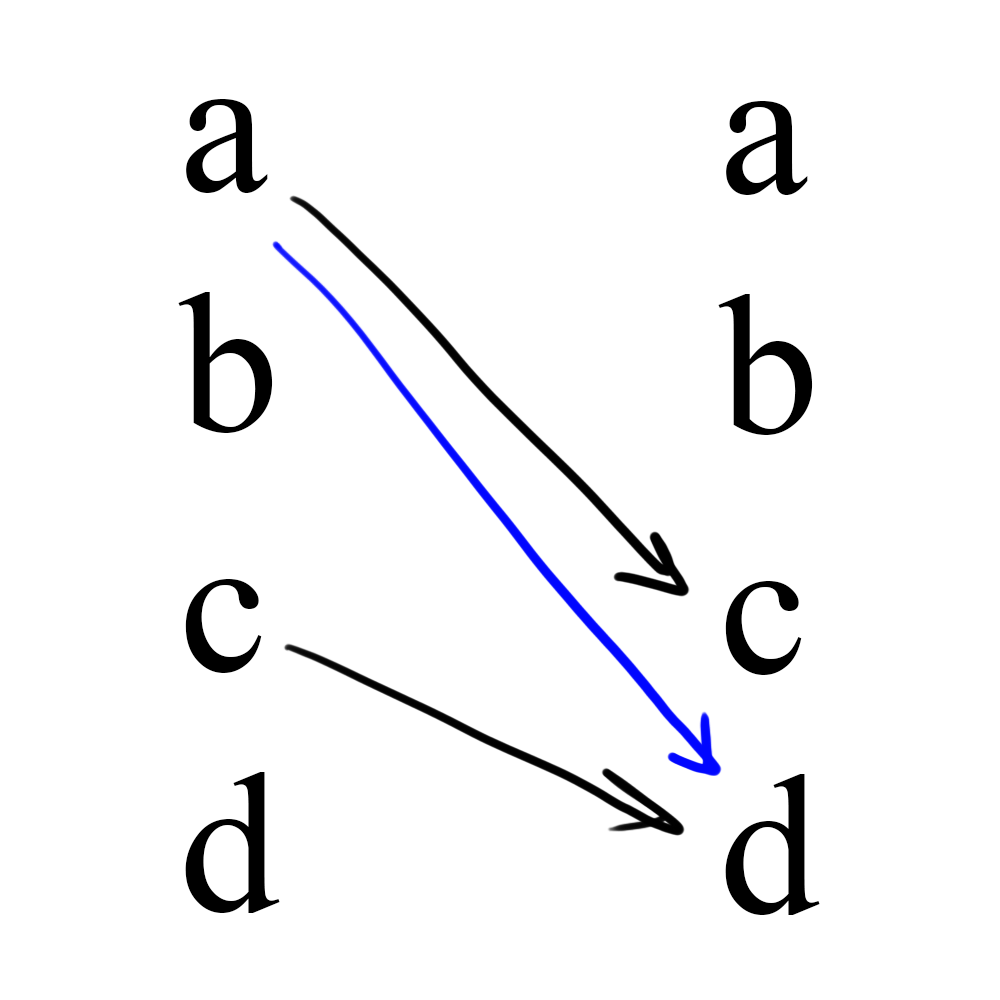
\includegraphics[scale=0.06]{s5}
  \caption[] {
    \tabular[t]{@{}l@{}}
    $ARS = (A, R)$
    \\ $A = \{a, b, c ,d\}$
    \\ $R = \{(a, c), (a, d), (c, d)\}$
    \endtabular}
\end{figure}

\begin{figure}[H]
  \centering
  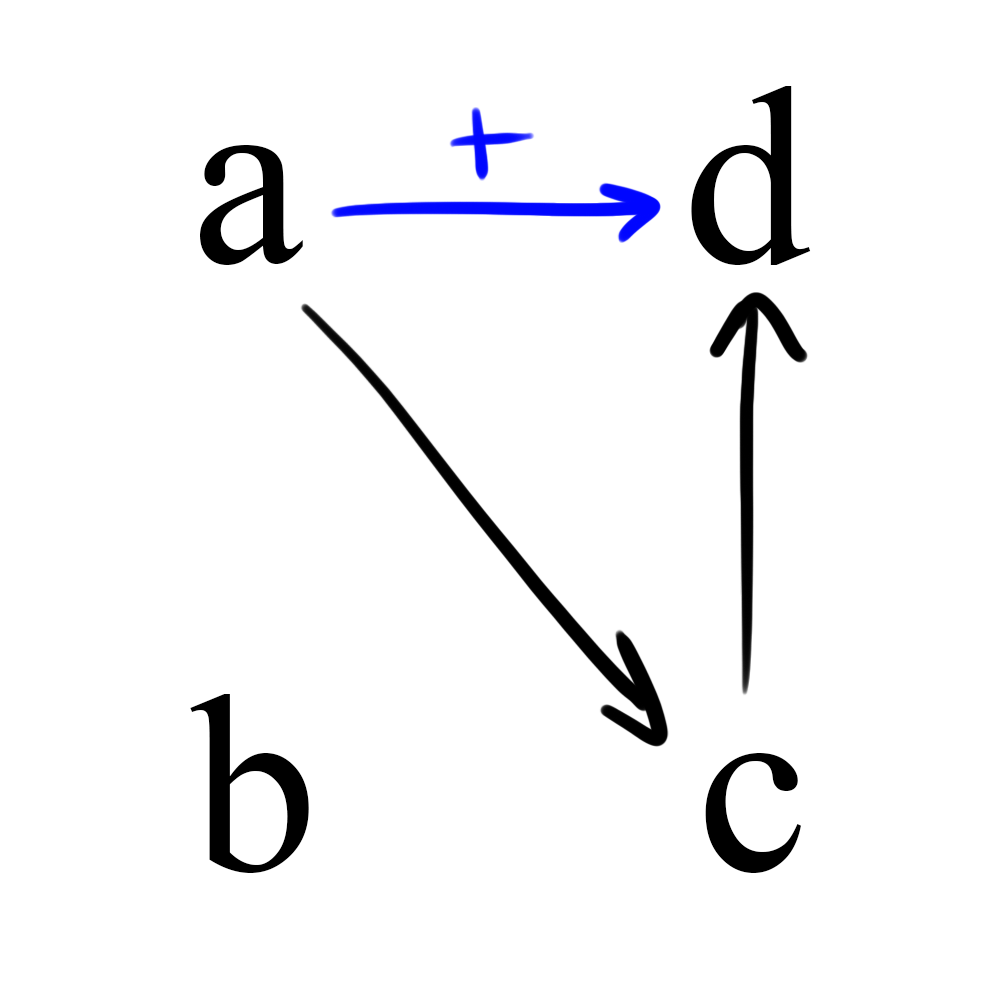
\includegraphics[scale=0.06]{v5}
  \caption[] {
    \tabular[t]{@{}l@{}}
    Traditional visualization of figure 24.
    \endtabular}
\end{figure}

\medskip\noindent
It is very important to keep in mind that the example we just covered was very basic. The ARS consisted of only one transitive relation which was $a \xrightarrow{+} d$. The whole ARS in this instance is transitive, because there are no other non-transitive relations between two objects. If we were to check if a more complex ARS was transitive, we would need to make sure there is a shortcut relation for every set of objects that require it, such as $a$ and $d$ which go through $c$.

\medskip\noindent
Similar to reflexive and symmetric ARS's, transitive ARS's share the sort of "all or nothing" type of requirement. Transitive ARS's require every instance of transitivity when given the chance, and if that is not the case, the ARS can not be transitive. In simpler words, there must be shortcuts between objects whenever possible in order for the ARS to be transitive. Going back to the bedroom/kitchen anology, there would have to be a shortcut hallway for every two rooms in a house, no matter how many rooms there are.


\section{Project}

\subsection{Introduction to Lindenmayer Systems}

\medskip\noindent
Lindenmayer systems, which also known as L-systems, are rewriting systems that can be used to visualize growth of plants or other fractal-like organic forms. These rewriting systems are directly related to the abstract reduction systems (ARS's) that we have already covered in the theory section of this report. That section contained many theoretical topics such as termination, UNF's, reflexivity, etc. This section will not only compare L-systems to ARS's, but will also explain how they work, what they look like, and how to make them aesethetically pleasing. The aspect of L-systems that many find appealing is that they can be used to visualize and create very beautiful patterns. The ones we will focus on are very similar to those found in plants such as trees, weeds, and ferns.

\medskip\noindent
It is extrememly helpful to use special software to draw these patterns. Drawing them manually can take ridiculous amounts of time depending on how many branches are desired. For this report, I will be using the software, \href{https://processing.org/Processing}{Processing}. Processing is a graphical library and IDE that allows developers to draw interesting patterns to the screen with nothing but code. It is built on top of Java and is also free. I highly recommend downloading it as there is much potential for visualization in general. With minor modificiations, I used Daniel Shiffman's Processing code from GitHub to test out and visualize different L-systems. You may access this very same code \href{https://github.com/nature-of-code/noc-examples-processing/tree/master/chp08_fractals/NOC_8_09_LSystem}{here}. For further reading on the endless possibilities of Processing, see Daniel Shiffman's book, \emph{The Nature of Code}, \href{https://natureofcode.com/}{here} \cite{NC}.

\subsection{Rules of Lindenmayer Systems}

\medskip\noindent
Unlike the ARS's that we have been working with, the rules within L-systems contain symbols that determine the direction of the branches. This allows for more control when visualizing the multiple complex paths they create. The prior ARS visualizations of this report do not have these special symbols. It was implied that the trees would branch downwards for the purpose of focusing on the theory. With L-systems, it is not only required but also very necessary to have these symbols to determine aspects such the tree shape and direction of growth. It is impossible to tell a computer how to draw a tree if it does not know what direction the branches should go. The new symbols are listed below:

\medskip
  $F$  = draw line forward

\smallskip
  $+$  =  rotate left

\smallskip
  $-$  =  rotate right

\smallskip
  $[$  =  begin new branch

\smallskip
  $]$  =  rotate right

\medskip\noindent
These symbols go within the rules portion of L-systems. Just like ARS's, L-systems have objects and rules too. We originally denoted ARS systems like the example below, where $A$ represented the objects of the system and $R$ represented the rules.

\medskip
  $ARS = (A, R)$

\smallskip
  $A = \{...\}$

\smallskip
  $R = \{...\}$

\medskip\noindent
To make the notation similar without getting confused, we will denote L-systems like in the example below, where $O$ represents the objects, and $R$ still represents the rules.

\medskip
  $L$-$sys = (O, R)$

\smallskip
  $O = \{...\}$

\smallskip
  $R = \{...\}$

\subsection{Lindenmayer System Example Walkthrough}

\medskip\noindent
Let's take a look at our first L-system example where:

\medskip
  $L$-$sys = (O, R)$
  
\smallskip
  $O = \{ F \}$
  
\smallskip
  $R = \{ (F \rightarrow F[+F]F[-F]) \}$

\medskip\noindent
First of all, it is important to address some of the differences from ARS's. A minor syntax difference is that we are now using "$\rightarrow$"s instead of commas in the rule ($R$) portion of the L-systems. This is just to create separation for readability. You may have also noticed that there are only one object and one set of rules. What is interesting about L-systems is that you can draw very complex patterns such as trees with simple systems. In fact, you can conceptualize them with ARS's. An ARS that would be very similar to the L-system above would be:

\medskip
  $ARS = (A, R)$
  
\smallskip
  $A = \{a\}$
  
\smallskip
  $R = \{(a, aa)\}$

\medskip\noindent
There are two key differences that you may have noticed between this ARS and the original L-system. The first is obviously the symbols. The second is that the L-system's rule, $R$, states that the object $F$ transforms into four more versions of itself. This seems to conflict the ARS's object, $a$, which only transforms into two versions of itself. The reason why this is the case is because $F$ is not only an object, but also the symbol for drawing a line forward. Therefore, drawing a line forward is really only noticable if there are new branches. If you look closely, you will find that the branches in the L-system are the same amount as the new objects in the ARS, if and only if you are counting $F$'s within branches ($[$ $]$'s) only. The other $F$'s simply draw lines forward to give the L-system more space to draw the new branches.

\medskip\noindent
Let us finally draw the L-system that we created above. Here is what the L-system looks like, being drawn what generation at a time, or one recursive loop at a time:

\begin{figure}[H]
  \centering
  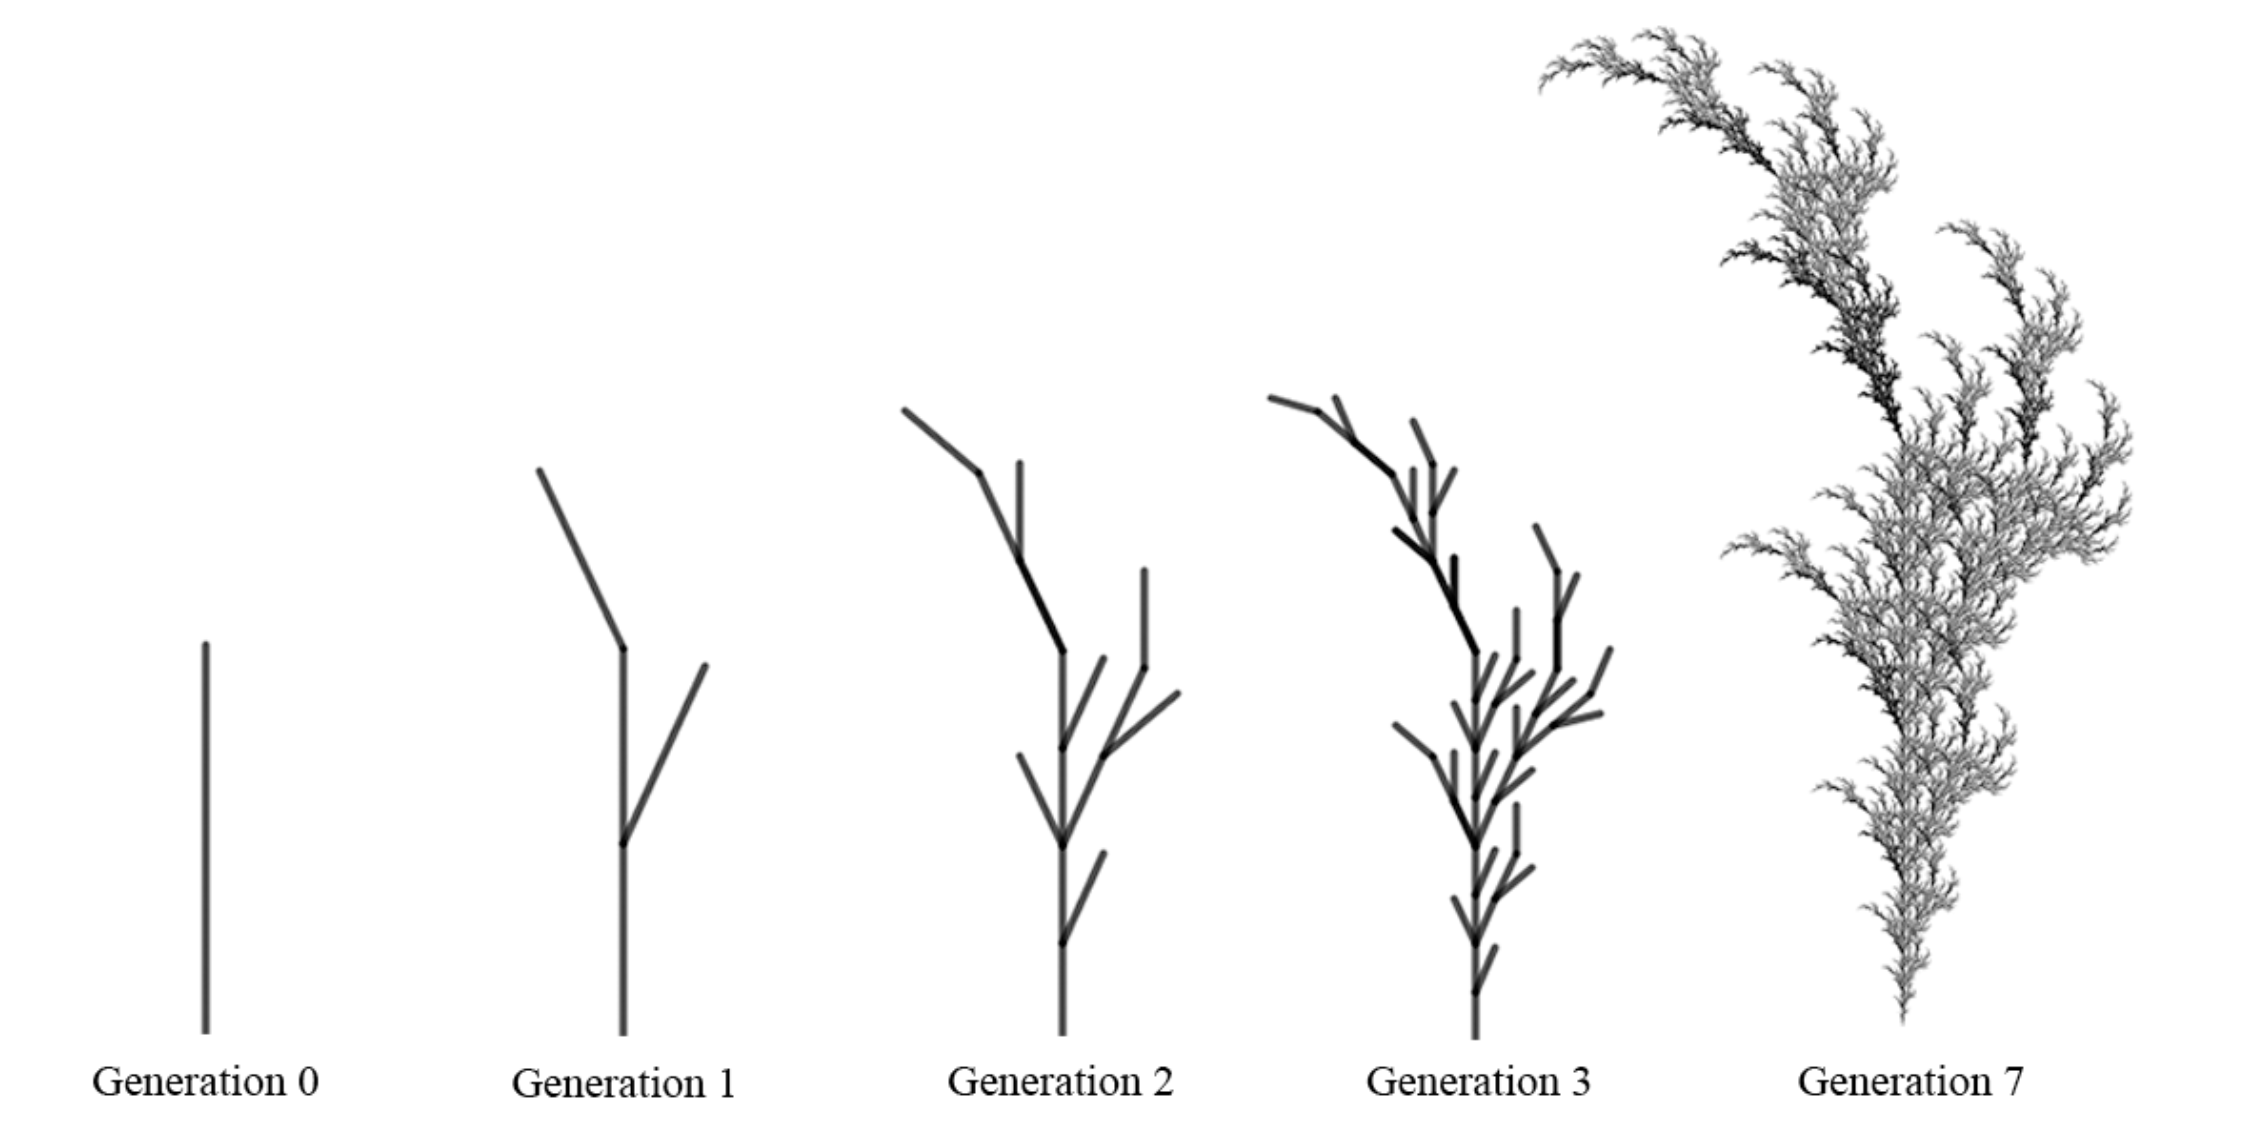
\includegraphics[scale=.3]{treeAs.PNG}
  \caption[] {
    \tabular[t]{@{}l@{}}
    $L$-$sys = (O, R)$
    \\ $O = \{ F \}$
    \\ $R = \{ (F \rightarrow F[+F]F[-F]) \}$
    \endtabular}
\end{figure}

\medskip\noindent
Above is the respective tree of the L-system. There are graphics for each generation. We will now focus on the rules that make the changes from generation 0-1. Generation 0 is a line because a this point only object $F$ exists which indicates that a line is drawn forward. In generation 1, another extension line is drawn forward which is denoted by $F$; it is hard to see because it is just a continuation of the previous line. Next, a new branch and line is drawn to the right ($[+F]$). After this, another line is drawn straight forward from the original path ($F$). Lastly, a final line is drawn to the left which is denoted by $[-F]$. In the following generations, the pattern recursively continues. It is important to keep in mind that the branches are not growing lower and lower from the trunk with each generation. It may look like this because the scale of the trees gets smaller for each generation. However, it is only possible for the trees to branch upward from pre-existing branch ends. Also, keep in mind that there is a variable in the Processing code that determines the turn angle.

\medskip\noindent
Of course, this L-system could keep branching on forever because it is recursive like an ARS. This ties back to  \hyperref[sec:PLT]{section three} and more specifically termination. The L-system is not terminating because it is recursively looping forever, and therefore there are no normal or unique normal forms. Furthermore, it is not confluent because the branches never converge back together. There is no valley. The rest of the L-systems will share these same properties.

\medskip\noindent
This first example is generally an unnatractive in the aspect that it does not really look like a tree or plant. To make something that appears a bit more organic, we will make the rules cautious of branching attractively.


\subsection{More Lindenmayer Examples}

\medskip\noindent
The following L-systems in figures 27 and 28 are similar to the first considering there is only one object and one respective rule \cite{LS}. However, the rules are a bit trickier. Though more complex, they will result in more realistic trees.

\begin{figure}[H]
  \centering
  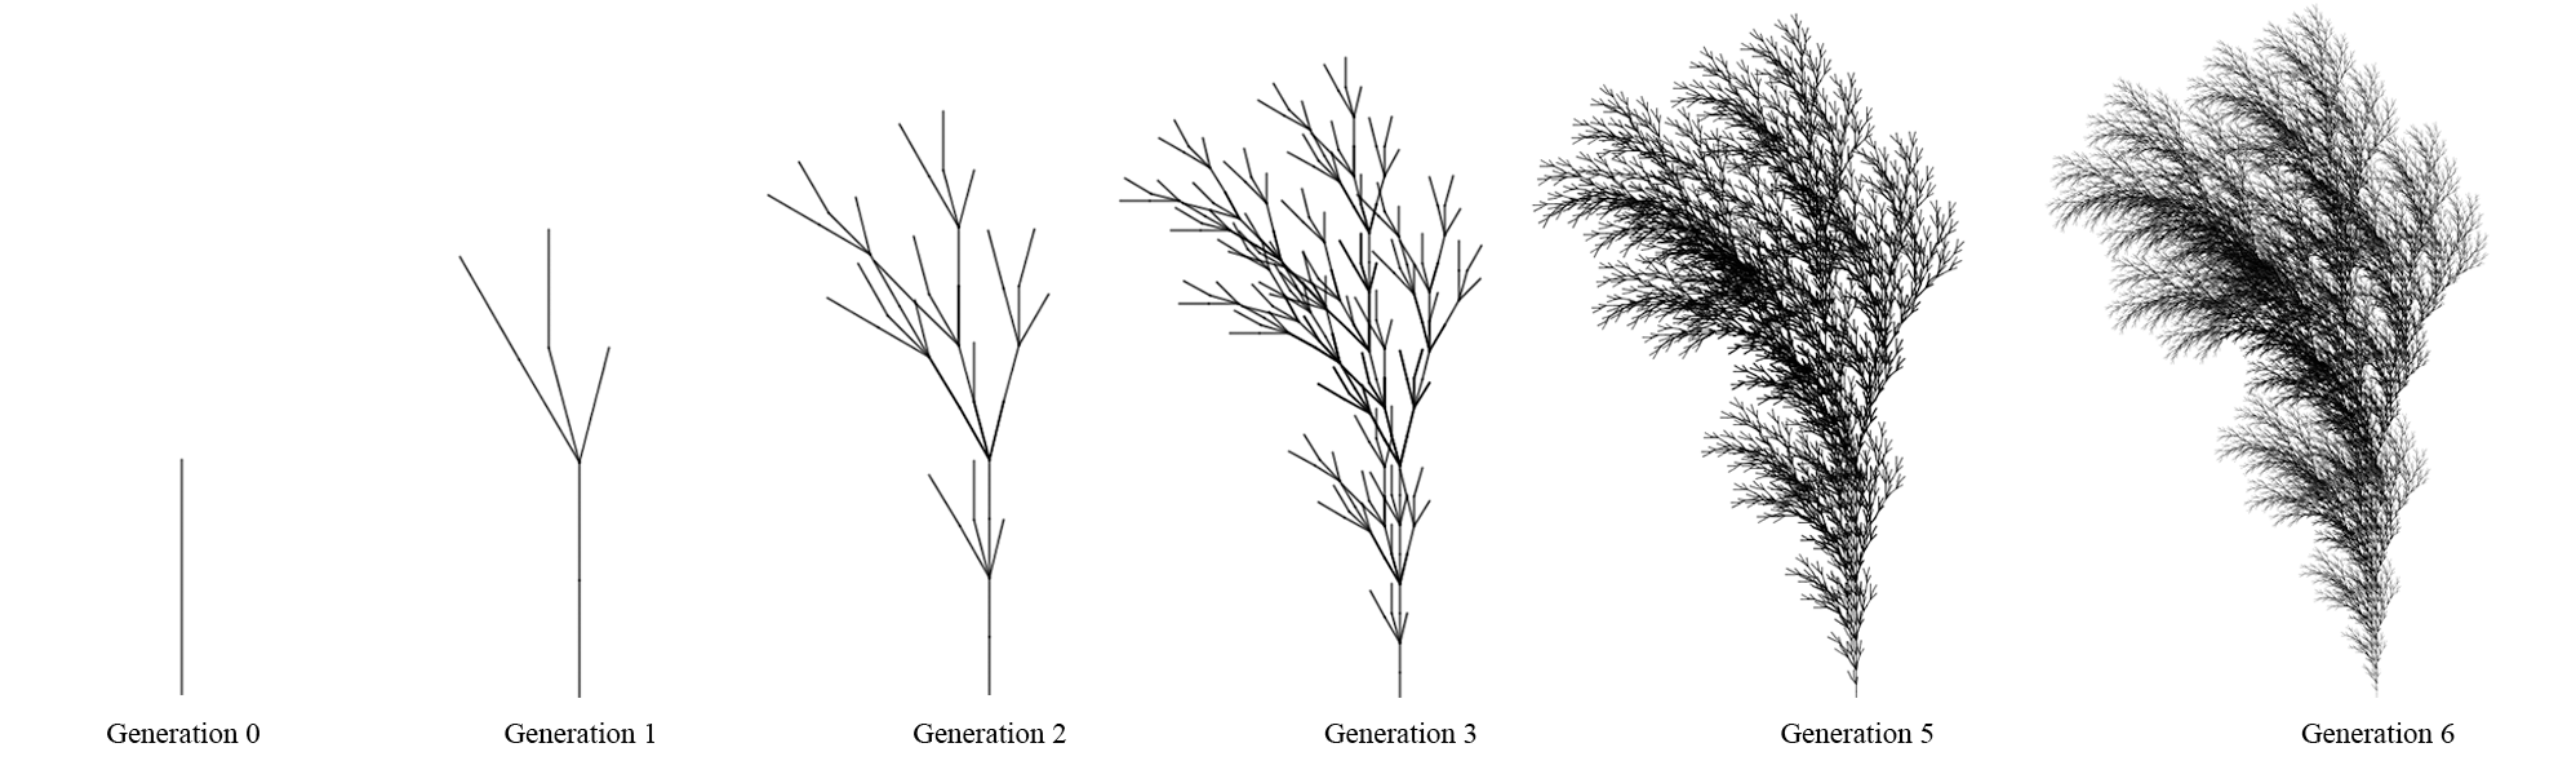
\includegraphics[scale=.3]{treeBs.PNG}
  \caption[] {
    \tabular[t]{@{}l@{}}
    $L$-$sys = (O, R)$
    \\ $O = \{ F \}$
    \\ $R = \{ (F \rightarrow FF[+F][--FF][-F+F]) \}$
    \endtabular}
\end{figure}

\medskip\noindent
You may notice that the rules, $R$ for figure 27's L-system contain more double $FF$'s. This is part of the reason why the trees look more natural. $FF$ allows for longer branches before fanning out since $F$ indicates drawing a line forward. Also, there are three new branches per recursive loop compared to the previous L-system which only had two.

\medskip\noindent
The mathematical equation that I found corresponds to the amount of $F$'s is listed in below. $x$ represents the generation.

\begin{equation}
  \resizebox{.18\hsize}{!}{$f(x) = \frac{3^{x+1}-1}{2}$}
\end{equation}

\medskip\noindent
However, it is rather difficult to correctly count the the amount of $F$'s. It is much easier to simply count the objects in an ARS. The corresponding ARS would be:

\medskip
  $ARS = (A, R)$
  
\smallskip
  $A = \{a\}$
  
\smallskip
  $R = \{(a, aaa)\}$

\medskip\noindent
The next L-system in figure 28 is similar to the previous example. The biggest key difference is that it leans to the right instead of the left. This is because there are more turn right signals, $+$ than turn left $-$. If you count these symbols in L-systems, you will find that whichever symbol is more present within the rules will determine which way the tree leans. If there are more $+$ symbols, it will lean right, and vise versa. This is because over multiple recursive loops many more branches are produced, and they generally go in the direction of the dominant symbol. This is because they branch off of each other. Without balance in an L-system, a tree can turn too much and sort of twist around. Here is the right leaning tree below:

\begin{figure}[H]
  \centering
  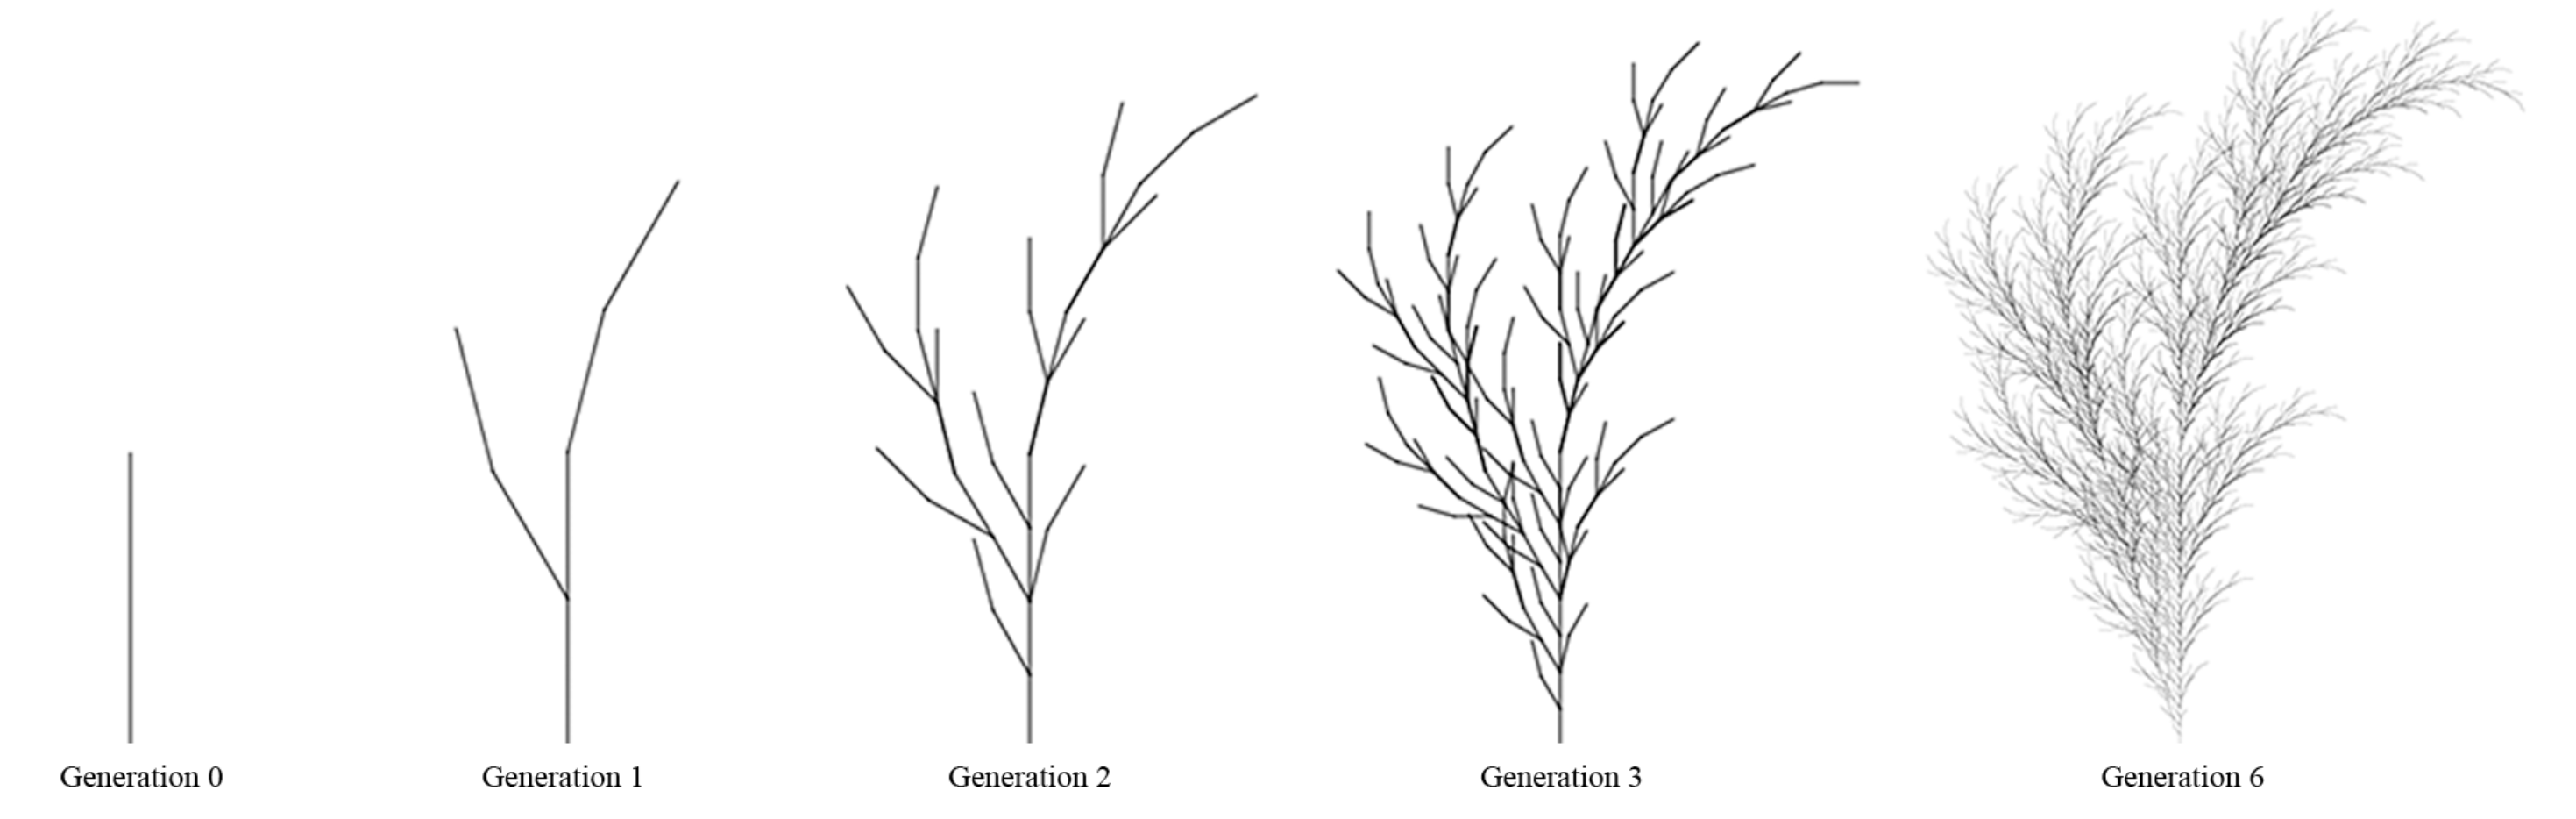
\includegraphics[scale=.265]{treeCs.PNG}
  \caption[] {
    \tabular[t]{@{}l@{}}
    $L$-$sys = (O, R)$
    \\ $O = \{ F \}$
    \\ $R = \{ (F \rightarrow F[--F[+F]]F[+F[+F]]) \}$
    \endtabular}
\end{figure}

\medskip\noindent
To visualize these L-systems in all of their glory, I reduced the line thickness and canvas size to make them much bigger. As they become even larger, they start to look like feather-like bushes or weeds. This is probably because these objects usually have more detail.

\begin{figure}[H]
  \centering
  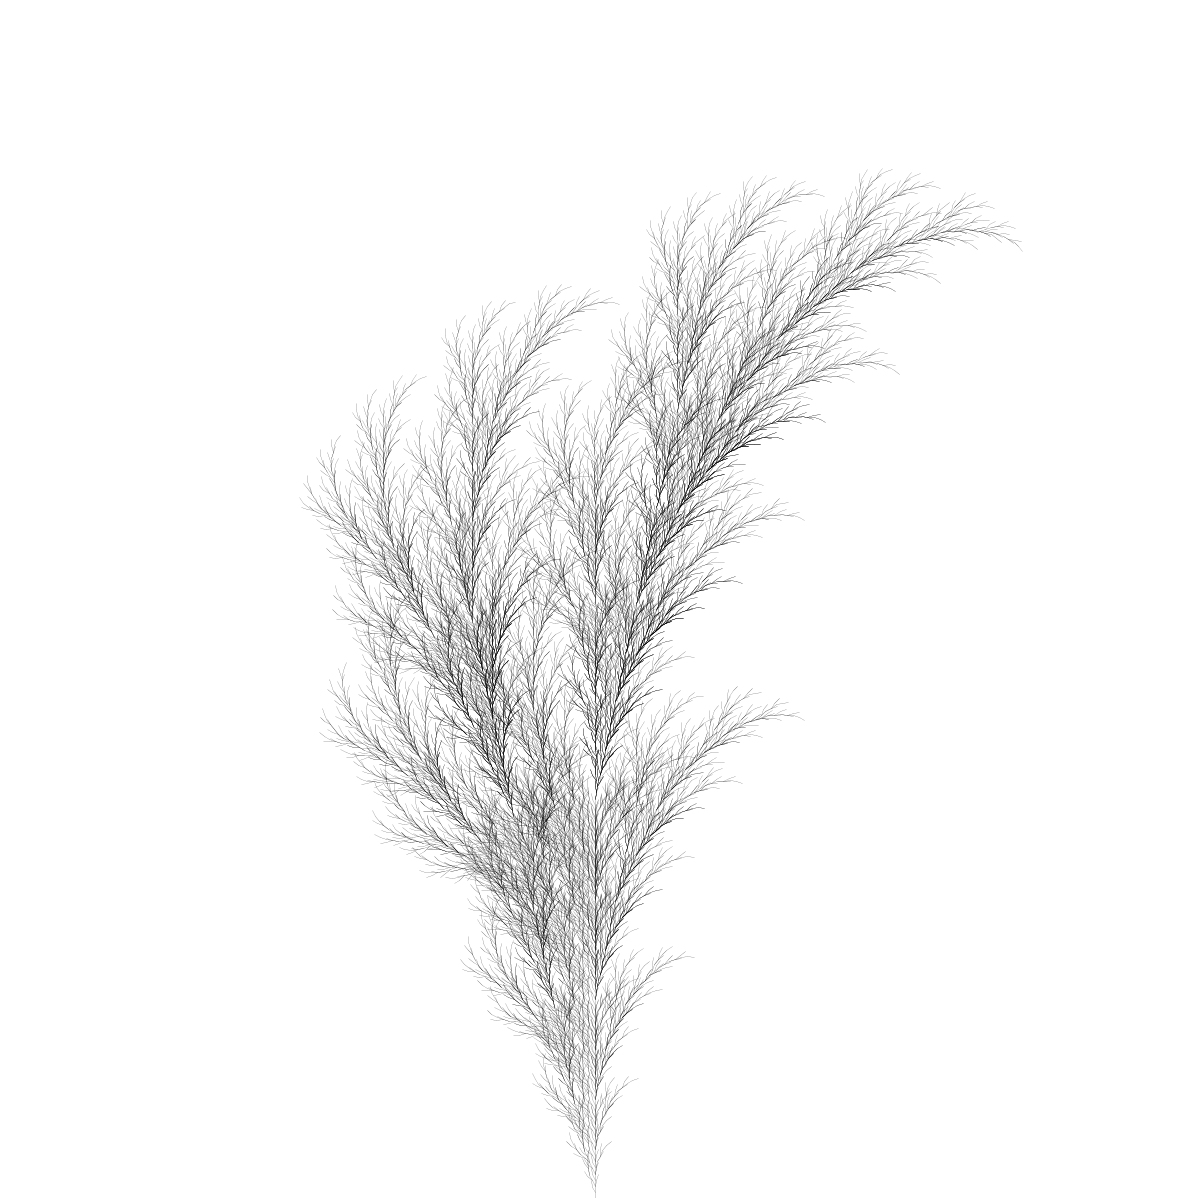
\includegraphics[scale=.4]{treeC8.PNG}
  \caption[] {
    \tabular[t]{@{}l@{}}
    Previous Example's Generation 7
    \endtabular}
\end{figure}

\begin{figure}[H]
  \centering
  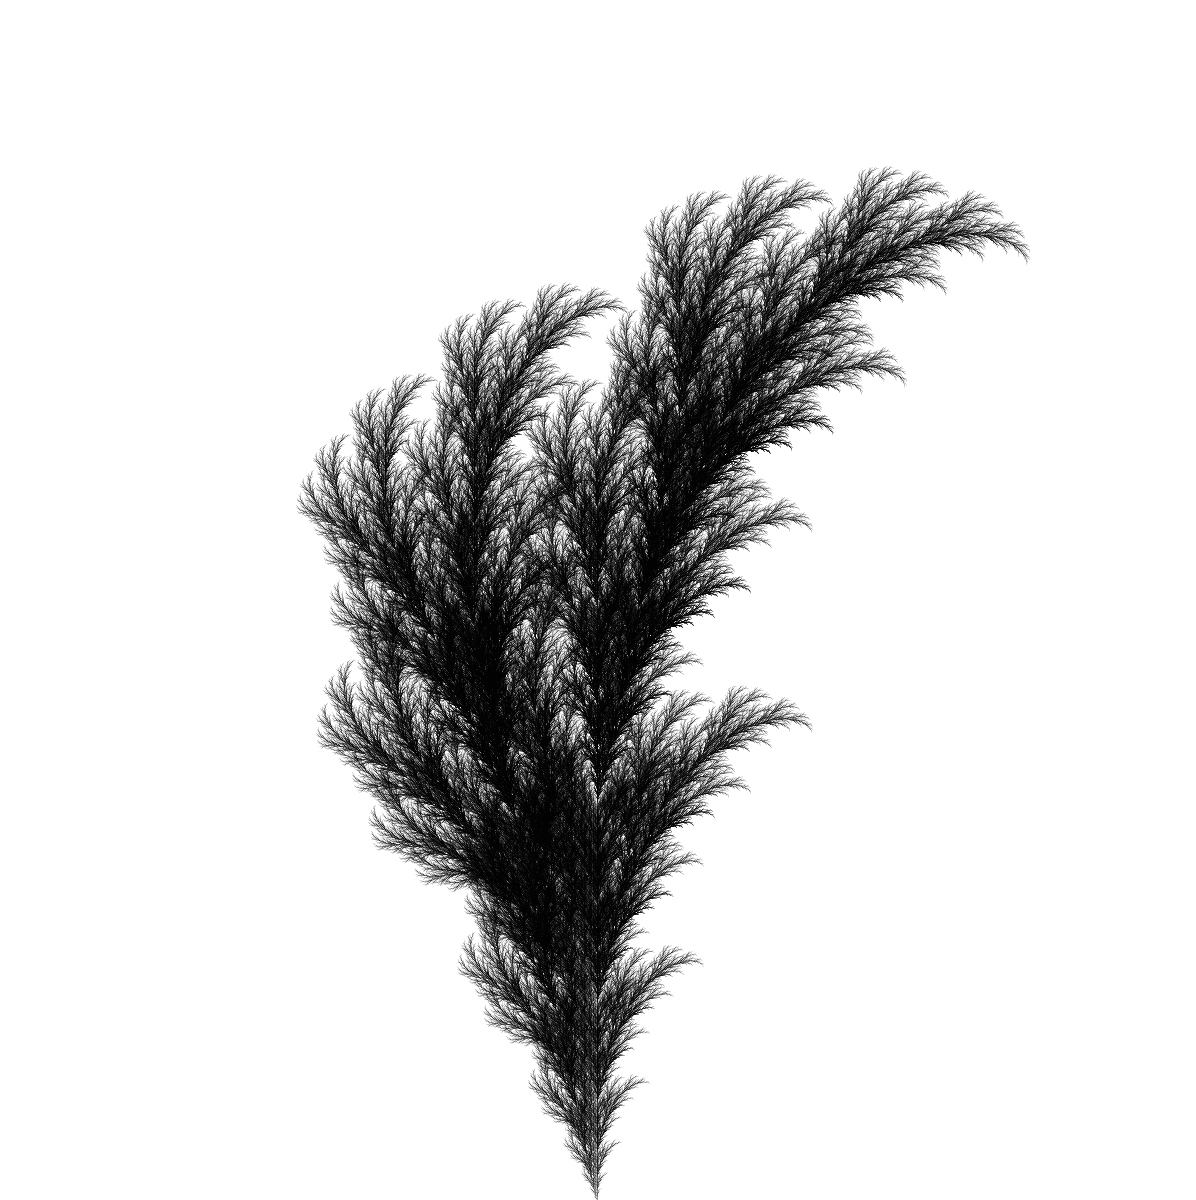
\includegraphics[scale=.5]{treeC9.PNG}
  \caption[] {
    \tabular[t]{@{}l@{}}
    Previous Example's Generation 9
    \endtabular}
\end{figure}

\medskip\noindent
As you can see, figure 30 appears very dark because there is much overlap of branches. This fills in much of the white space making some of the tree to appear as solid black. What is interesting about this is that if you stare at the figure long enough, there is a bit of an optical illusion where the white gaps in between the branches start to look like leaves of a plant. This may be more of just illusion than a theoretical or computational speculation but it is still interesting that even the whitespace between the branches can appear somewhat organic too.

\section{Conclusions}\label{conclusions}
At the beginning of this report, we explored Haskell by working with small examples. We differentiated both syntax and theoretical differences between imperative C code and functional Haskell Code. Some of the different Haskell material covered was variables, types, functions, recursion and pattern matching. To dive deeper into the theory of functional programming, we next dove into string rewriting and abstract reduction systems. Properties such as termination, unique normal forms, and confluence were covered. Also, the relationships between all of these and the conflicts between them were discussed in detail too. To conclude this theory portion of the report, reflexivity, symmetry, and transitivity were all studied using a two-column system of visualization. For the final part of the report, Lindenmayer Systems were covered. The similarities and differences between these L-systems and ARS's were discussed along with explanations about the uniqueness of L-system rules. These L-systems were visualized using software called Processing. Hopefully this report will encourage and fascilitate critical thinking for these various topics. I know that it was very effective in improving my understanding of programming languages in general.

\begin{thebibliography}{99}

\bibitem[PL]{PL} \href{https://github.com/alexhkurz/programming-languages-2021/blob/main/README.md}{Programming Languages 2021}, Chapman University, 2021.

\bibitem[LS]{LS} \href{https://www.erase.net/projects/l-systems/}{Project: L-Systems}, Erased, 2020.

\bibitem[LE]{LE} \href{https://wiki.haskell.org/Lazy_evaluation}{Lazy Evaluation}, Haskell Wiki, 2021.

\bibitem[HP]{HP} \href{https://wiki.haskell.org/Pure}{Pure}, Haskell Wiki, 2021.

\bibitem[RI]{RI} \href{https://hackmd.io/@alexhkurz/BJ7AoGcVK}{Rewriting: Introduction}, Alexander Kurz, 2021.

\bibitem[SRE]{SRE} \href{https://hackmd.io/@alexhkurz/Syn23oMHF}{String Rewriting Exercises}, Alexander Kurz, 2021.

\bibitem[RST]{RST} \href{https://www.youtube.com/watch?v=6fwJj14O_TM}{Reflexive, Symmetric, Transitive Tutorial}, LearnYouSomeMath, 2018.

\bibitem[ID]{ID} \href{https://learntocodetogether.com/imperative-vs-declarative-programming/}{Imperative vs. Declarative Programming}, Learn To Code Together, 2019.

\bibitem[HI]{HI} \href{https://www.youtube.com/watch?v=Vgu82wiiZ90&list=PLe7Ei6viL6jGp1Rfu0dil1JH1SHk9bgDV&index=1}{Haskell for Imperative Programmers}, Philipp Hagenlocher, 2020.

\bibitem[NC]{NC} \href{https://natureofcode.com/}{The Nature of Code}, Daniel Shiffman, 2012.

\bibitem[PM]{PM} \href{https://stackoverflow.com/questions/2225774/haskell-pattern-matching-what-is-it}{Pattern Matching}, Stack Overflow, 2010.

\bibitem[FAC]{FAC} \href{https://stackoverflow.com/questions/2225223/guarded-equations-in-haskell}{Guarded Equations in Haskell}, Stephan202, 2010.

\bibitem[DD]{DD} \href{https://techdifferences.com/difference-between-definition-and-declaration.html}{Definition vs. Declaration}, TechDifferences, 2021.

\bibitem[HR]{HR} \href{https://en.wikibooks.org/wiki/Haskell/Recursion}{Haskell/Recursion}, WikiBooks, 2020.

\end{thebibliography}

\end{document}